% 
%%
%% Copyright 2007, 2008, 2009 Elsevier Ltd
%%
%% This file is part of the 'Elsarticle Bundle'.
%% ---------------------------------------------
%%
%% It may be distributed under the conditions of the LaTeX Project Public
%% License, either version 1.2 of this license or (at your option) any
%% later version.  The latest version of this license is in
%%    http://www.latex-project.org/lppl.txt
%% and version 1.2 or later is part of all distributions of LaTeX
%% version 1999/12/01 or later.
%%
%% The list of all files belonging to the 'Elsarticle Bundle' is
%% given in the file `manifest.txt'.
%%

%% Template article for Elsevier's document class `elsarticle'
%% with numbered style bibliographic references
%% SP 2008/03/01
%%
%%
%%
%% $Id: elsarticle-template-num.tex 4 2009-10-24 08:22:58Z rishi $
%%
%%
\documentclass[preprint,12pt,3p]{elsarticle}

%% Use the option review to obtain double line spacing
%% \documentclass[preprint,review,12pt]{elsarticle}

%% Use the options 1p,twocolumn; 3p; 3p,twocolumn; 5p; or 5p,twocolumn
%% for a journal layout:
%% \documentclass[final,1p,times]{elsarticle}
%% \documentclass[final,1p,times,twocolumn]{elsarticle}
%% \documentclass[final,3p,times]{elsarticle}
%% \documentclass[final,3p,times,twocolumn]{elsarticle}
%% \documentclass[final,5p,times]{elsarticle}
%% \documentclass[final,5p,times,twocolumn]{elsarticle}

%% if you use PostScript figures in your article
%% use the graphics package for simple commands
%% \usepackage{graphics}
%% or use the graphicx package for more complicated commands
%% \usepackage{graphicx}
%% or use the epsfig package if you prefer to use the old commands
%% \usepackage{epsfig}

%% The amssymb package provides various useful mathematical symbols
\usepackage{amssymb}
\usepackage{graphicx}
\usepackage{subcaption}
%% The amsthm package provides extended theorem environments
%% \usepackage{amsthm}

%% The lineno packages adds line numbers. Start line numbering with
%% \begin{linenumbers}, end it with \end{linenumbers}. Or switch it on
%% for the whole article with \linenumbers after \end{frontmatter}.
%% \usepackage{lineno}

%% natbib.sty is loaded by default. However, natbib options can be
%% provided with \biboptions{...} command. Following options are
%% valid:

%%   round  -  round parentheses are used (default)
%%   square -  square brackets are used   [option]
%%   curly  -  curly braces are used      {option}
%%   angle  -  angle brackets are used    <option>
%%   semicolon  -  multiple citations separated by semi-colon
%%   colon  - same as semicolon, an earlier confusion
%%   comma  -  separated by comma
%%   numbers-  selects numerical citations
%%   super  -  numerical citations as superscripts
%%   sort   -  sorts multiple citations according to order in ref. list
%%   sort&compress   -  like sort, but also compresses numerical citations
%%   compress - compresses without sorting
%%
%% \biboptions{comma,round}

% \biboptions{}


\journal{Computers \& Education}

\begin{document}

\begin{frontmatter}

\title{The conception of parameters and constraint based models in architectural projects: the case of Lel\'e's pivot domes}





\begin{abstract}

Following the increasing interest form architects on the application of generative algorithms in conception of projects, many questions have been raised about teaching this particular way of thinking about forms. One of the main goals on learning the subject is to understand how an idea of a construction element can be translated in to the rules of an algorithm. Others are: to introduce concepts of programming necessary to implement the algorithms and to place this methods in the scope of disciplines involved in the construction activity. This paper propose a example based strategy to discuss this three crucial points, using the pivot domes designed by Brazilian architect Lel\'e as an object of study. 

\end{abstract}

\begin{keyword}
%% keywords here, in the form: keyword \sep keyword
Parametric Models \sep Geometric Constraints \sep Generative Algorithms.
%% MSC codes here, in the form: \MSC code \sep code
%% or \MSC[2008] code \sep code (2000 is the default)
\end{keyword}

\end{frontmatter}

%%
%% Start line numbering here if you want
%%
% \linenumbers

%% main text
\section{Introduction}
\label{sec1}

The concepts, techniques and applications of generative algorithms has gain, in the passing of the last decades, a great amount of attention form architectural practices, researchers and teachers \cite{krish2011}. Many of the global leading \textit{bureaus} in the field of Architecture have invested in implementing and maintaining a programming department to collaborate in the creative process of building design \cite{ceccato2010mbg}. The range of influence of the computer-aided design (CAD) extrapolate the aspect of an applied tool and reaches the aesthetic theories \cite{Oxman2006} \cite{picon2011} and, considering the integration with computer-aided manufacturing (CAM) systems, the construction activities \cite{kolarevic2003}. The generative algorithm contributed with it's share in this process.

In the academic world, the assimilation of the methods, tools and knowledge involved in the understanding of the generative design paradigm, grants, from representing a great challenge, a latitude of possibilities and an opportunity to rethink the relations among disciplines involved in the process \cite{kolarevic2003} \cite{aag2010113}.

One of the main issues on teaching generative design to novice users is to make them understand how an initial idea can be translated in rules that generate forms. The understanding of how this forms could be generated is the first step into this different way of approaching the project activity that this algorithms embrace. It's important to remember that this generation of forms in not an objective in itself, but a tool to assist the answering of questions raised form the point of view of the Architecture as an interdisciplinary domain. In that sense, the building of effective generative algorithms also relies in the understanding of witch characteristics of the building or construction element may be explored and tested by the process. How different parameter will act together in a way that the variant forms generated by those will establish a set of possible solutions, each one with particular characteristics, to be disposed or adopted by the user.

This paper proposes a example-based strategy to introduce the generative algorithms student in the definition of the rules that governs a conceptual model of an architectural element based on parameters and constraints. In the interdisciplinary scope, the geometrical constructions used, concepts on list manipulation based programming and aesthetics aspects of the generated forms are also presented and discussed.


\section{Generative design and generative algorithms}
\label{generaalgor}

Algorithms are defined as a finite set of rules that describes the steps do solve an specific problem \cite{knuth1997art}. The technical draw applied in the design of architectural plans are, indeed, algorithms \cite[chap. 3]{terzidis2006algorithmic} , and the sequential operations with compass, rule and straightedges, used to make any of the geometric constructions, describes it's rules. Words like "perpendicular", "parallel" and "tangent" summarize entire algorithms in the debates that orbit the project activity. The development of CAD technology, started by providing the ability to reproduce this drawing algorithm to the software, and them evolving from that to a "wider graphic vocabulary available to designers, together with a more elaborate syntax---in all, a richer and potentially more expressive graphic and spatial language" \cite[chap. 15]{mitchell2008}.

\begin{figure}[!h]
\begin{center}
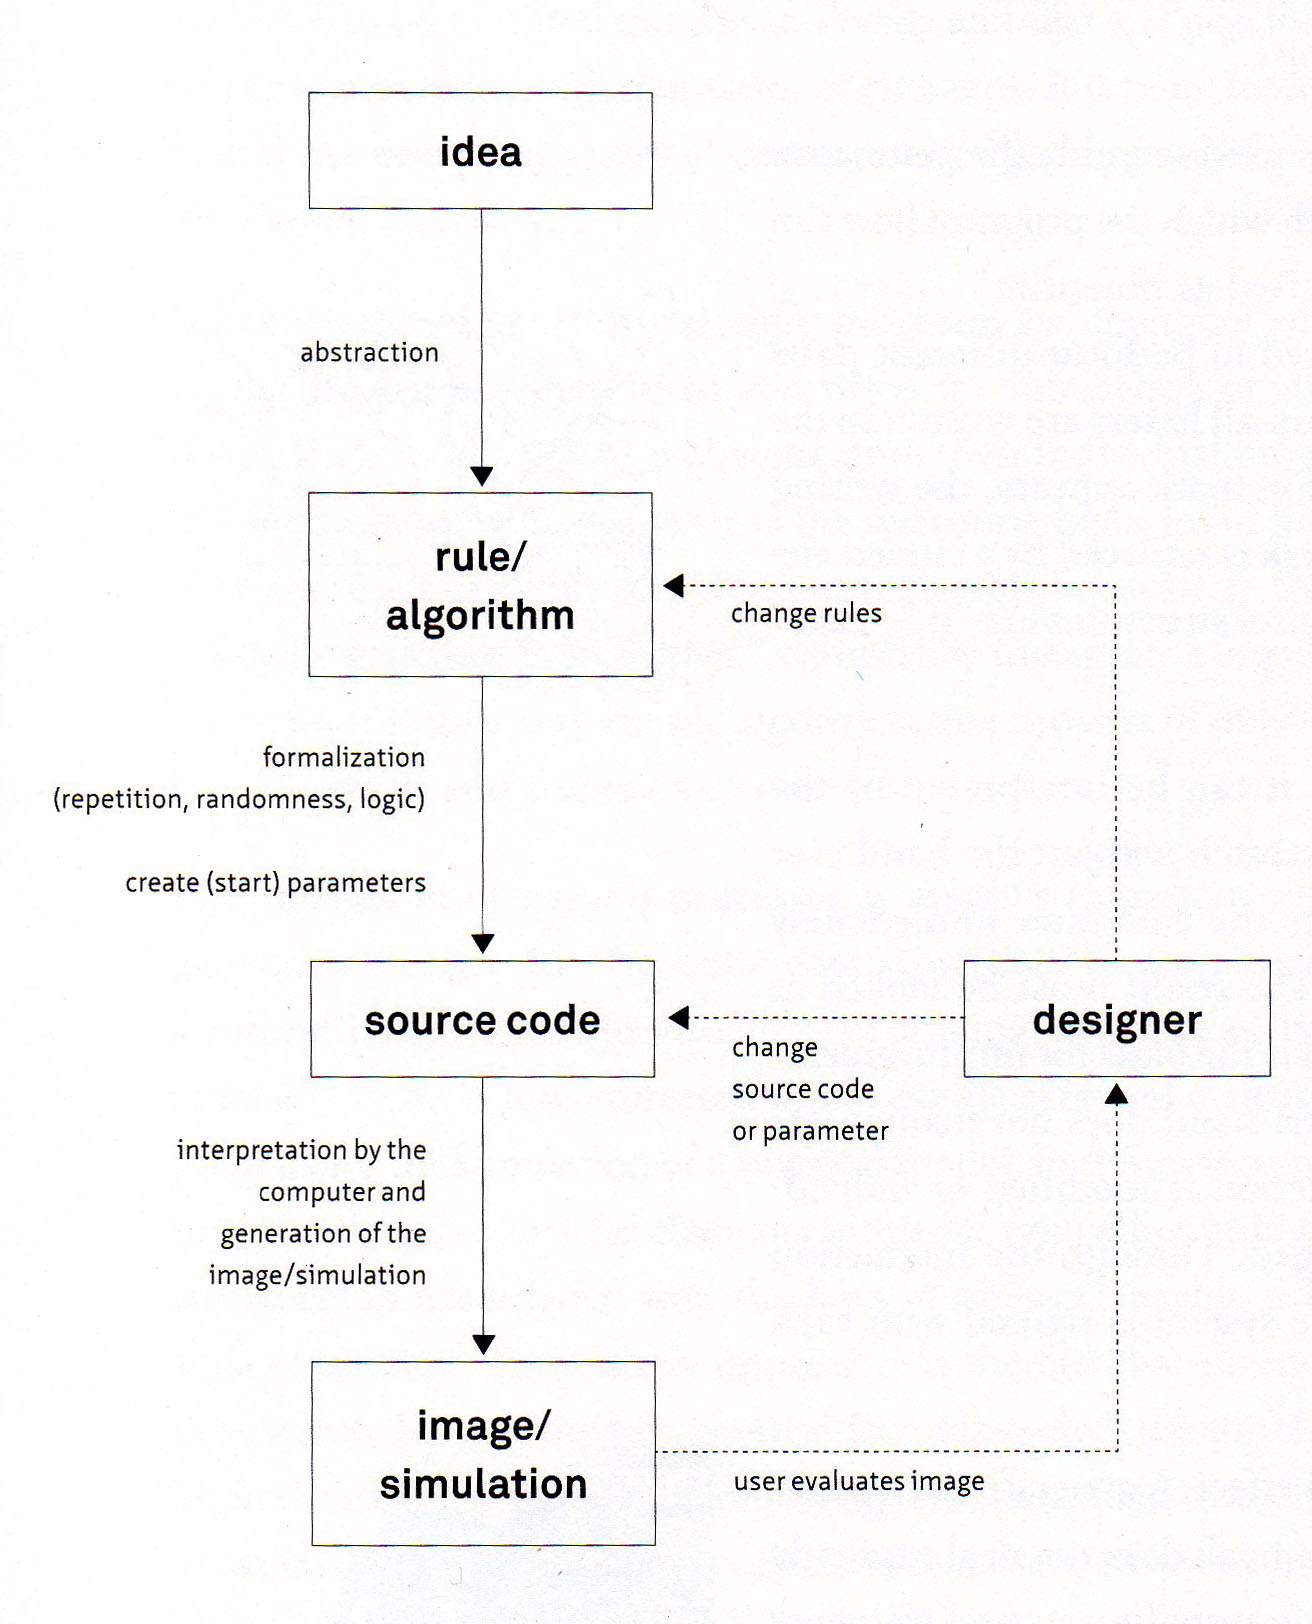
\includegraphics[width=0.5\textwidth]{fluxogramametodologia.jpg}
\caption{Flowchart of a generative algorithm }
\label{figura:fluxogramametodologia}
\end{center}
\end{figure}

Generative Design, in a broad definition, is the application of algorithms or a " rule based process through which various potential design solutions can be created " \cite{fasoulaki2008} and the generative algorithms are the logical engine propelling that design strategy in the computational context. As stated before, all the technical draw constructions are algorithms. The variety an variants of buildings designed by those methods are unmeasurable. The generative design techniques differs from the traditional methods for transforming the methodology of work. The generative systems provides a degree of automaticity to the process, enabling the user to evaluate a greater number of possible solutions to the architectural problem in a shorter amount of time than it wold be possible to do by the traditional methods.


In Fig. \ref{figura:fluxogramametodologia} \cite{bohnacker2012} a flowchart illustrates the process of creating an operating an generative algorithm in a elucidative way. The real shift promoted by the generative algorithms are in the process of electing the form to be constructed. Starting with an idea of what should be the constructed object, as an abstraction that is translated in a set o rules. An algorithm is implemented in a programming language, code or a visual programmable ambient, obeying the rules and a simulation of the model is generated by setting the parameters values and running the algorithm. The designer evaluates the output and, by changing the parameters values, the rules and/or the code, generates different outputs and chooses the final solution among those. The construable artifact appear only when the designer elect the proposal to be build \cite{DIno2012}.

Many computational methods where applied in the creation of  forms driven by generative algorithms: shape grammars \cite{stiny1972} \cite{Stiny1978} \cite{duarte2005} \cite{tepavcevic2012}, genetic algorithms \cite{caldas1999} \cite{fasoulaki2008} \cite{Troiano2012} \cite{Caldas2002}, cellular automata  \cite{Herr2007}, simulated annealing \cite{Ceranic2001} \cite{Correia2001} \cite{Lamberti2008}, tabu search \cite{Bland1991}, swarm intelligence \cite{Luh2011} \cite{Yahya2014} and parametric models \cite{Turrin2011} \cite{Fischer2005} \cite{lachauer2011a} \cite{Milena2010a} among others.

\section{Parameters and constraints based models (PCM)}
\label{ParamConst}

All generative algorithms, as well all the computer processing, are based in parameters, although the parametric design differentiate from the others by emphasizing the manipulation of parameters \cite{DIno2012}. For drawing a right prism in a cad system, the user has to input values for the width, height and depth. In a parametric design system, every one of this inputs can be modified interactively, and the prism dimensions will be automatically updated in the drawing.

Among many computer simulation methods to implement a generative design system, the constraint solver, since it´s introduction, by Pro/Engineer in the 1980's and it´s adoption by most of the available cad systems \cite{Hoffmann2005}, has gain attention by the intuitive and fluid manipulation of the forms calculated by this kind of solver. The methods relays on constraint problems satisfaction, consisting of, in a finite set of variables, each of those assigned to a finite domain and having the values that can be taken together restricted by constraints, finding a combination of this values that satisfies all the constraints \cite{Bartk01theoryand}. The definition of parameters and constraint based models here proposed is a way of emphasize both the parameters and the constraints that conducts a generative design process. 

The creation and manipulation of geometric forms in an ambient that enable the use of a constraint solver is tightly related to geometric theorem proving \cite{Hoffmann2005}. Geometry is a cornerstone in Architecture and construction since the early History of those fields \cite{ceccato2010mbg}, and the teaching of generative algorithms should explore the geometric knowledge from an alternative point of view.  

\section{Object of study}
\label{obstudy}

The Brazilian architect Jo\~ao Filgueiras Lima, better known by the nickname of Lel\'e, is one of the most important and celebrated architects of the country \cite{ARQ:359533}. Considered by Oscar Niemeyer a " great master of architecture ", and by Lucio Costa " the architect in whom art and technology meet and merge " \cite{ferraz2000joão}. His works reveals a strong interest in rationalization in the use of materials, an outstanding development of prefabrication and environmental integration, adopting daylight and air circulation innovatory solutions \cite{Campagnol2014}
 \cite{Maciel2007}.

\begin{figure}[!h]
\begin{center}
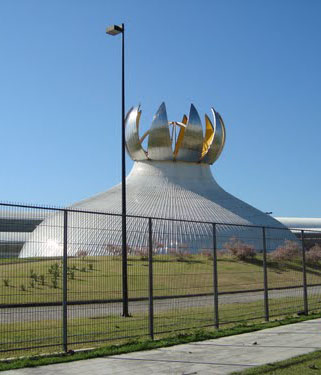
\includegraphics[width=0.3
\textwidth]{sarahcupula.jpg}
\caption{Sarah Hospital auditorium, Rio de Janeiro - RJ  -  www.sarah.br}
\label{figura:sarah}
\end{center}
\end{figure}

As an object of study, the pivoting domes used in the auditorium of the Sarah Kubitschek Hospital in Rio de Janeiro (Fig. \ref{figura:sarah}) and in two buildings of the proposal for the Labor Justice Courthouse complex, in the city of Salvador - Ba. In Figure \ref{figura:trt}, a 3D model of the complex presents the dome of the auditorium open in the right and the dome of the main court closed in the left.


\begin{figure}
\begin{center}
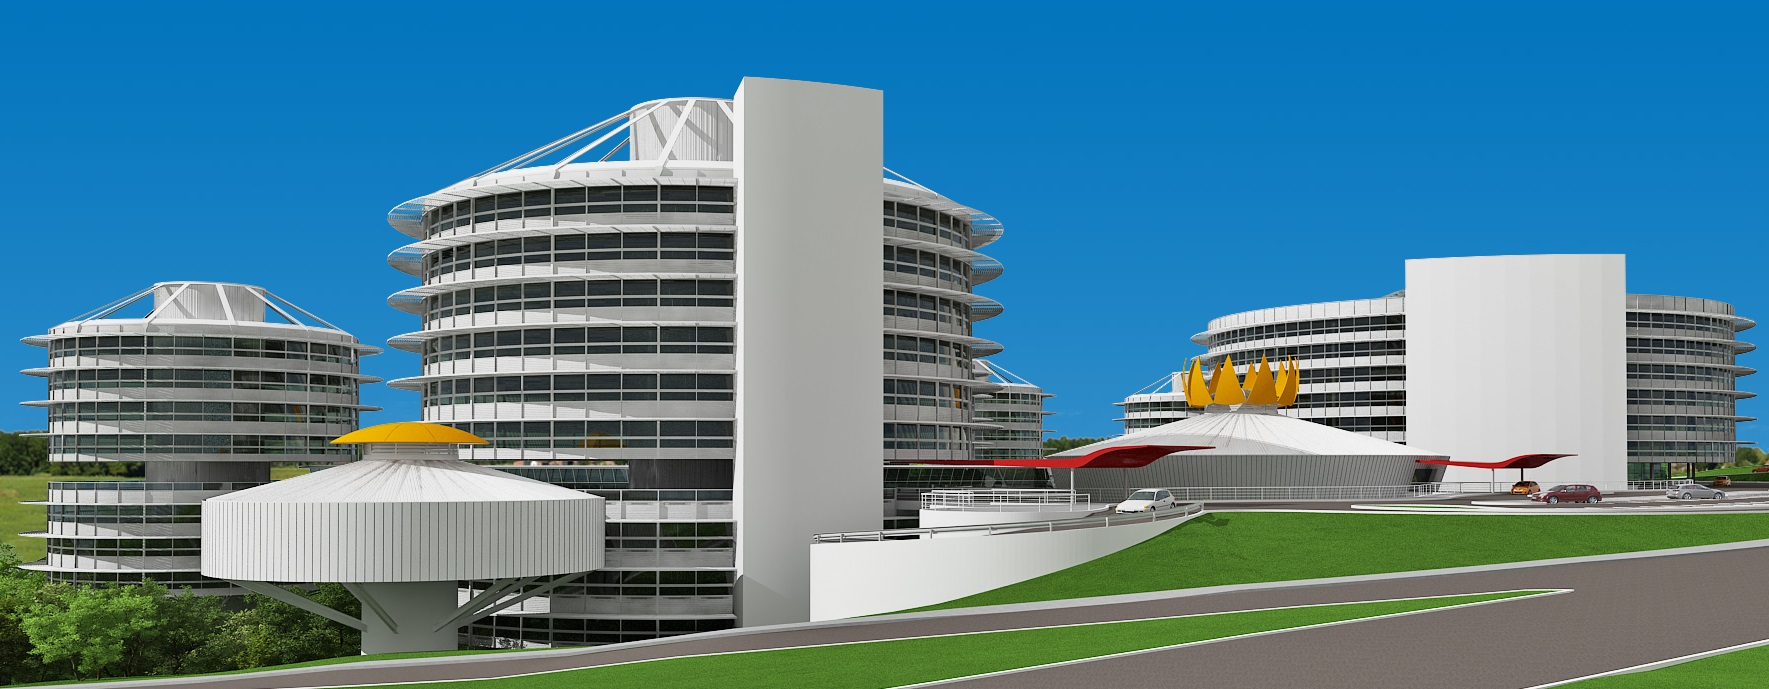
\includegraphics[width=0.7
\textwidth]{trt.jpg}
\caption{Labor Justice Courthouse Complex, Salvador - Ba source: Instituto Habitat archives}
\label{figura:trt}
\end{center}
\end{figure}

The first box in the flowchart in Figure \ref{figura:fluxogramametodologia} represents the idea of the family of forms to be generated. There are didactic advantages on presenting image references to illustrate the idea behind the generative algorithms to be build. In stead of describing an abstract idea of a goal, the architectural examples clarify important aspects of the intended solution. The application of this elements in real projects, the aesthetic composition that emerged from the variant forms of the domes and their relation whit the buildings that they are a part of, and the fact that many aspects of the algorithm can be visually identified could be also mentioned. A discussion about an "one sentence definition of the idea" could be conducted in class, or this sentence could be proposed by the teacher. The summarized idea should point the students attention to the goals of the algorithm in study. "A dome, divided in petals that pivot around axes on their base" is a good example of the idea's definition.


\section{Defining the parameters}
\label{implem}

Starting from the idea, the pivoting domes presented in Figures \ref{figura:sarah} and \ref{figura:trt} should be translated in algorithms that can automatically draw variations of those forms. Analyzing the domes presented in the Figures \ref{figura:sarah} and \ref{figura:trt}, the similarities and differences between the elected solutions can be listed:

\begin{itemize}
\item all the domes are , when closed, spherical caps;
\item the number of petals in the presented examples are different;
\item the base radius and height of the spherical cap, in the presented examples, are different;
\item the base of the petals are on the base of the spherical cap;
\item the top of the petals are on the maximum height of the sphere.
\end{itemize}

Based on this visual observations, many elements of the algorithm can be defined. The parameters, for instance, can be the \textbf{base radius}, the \textbf{center point} of the base, the maximum \textbf{height} and the \textbf{number of petals}. Another parameter should be added to the algorithm to simulate the pivoting movement of the dome: a \textbf{rotation angle} parameter.

Is important to note that other parameters could replace the elected ones to draw the same forms. The radius of the full sphere, the difference between the cap height and the center of the sphere, for example, could replace the maximum \textbf{height}, the base \textbf{center point} and the cap base \textbf{radius} generating the same geometries. Although equivalent results can be accomplished by the both strategies, it´s a good practice to think about what characteristics of the construction element are intended to be explored and how the parameters to be manipulated will fit in the process. Assuming that, in the presented example, the main characteristics to be explored are: the area of illumination and ventilation provided by the dome when opened and the aesthetic relation between the radius and the maximum height. That assumption justifies the proposed parameters as they directly operate on the characteristics on focus.


\section{Geometric constructions and constraints}
\label{geometric}

\begin{figure}
\begin{subfigure}{0.3\textwidth}
  \centering
  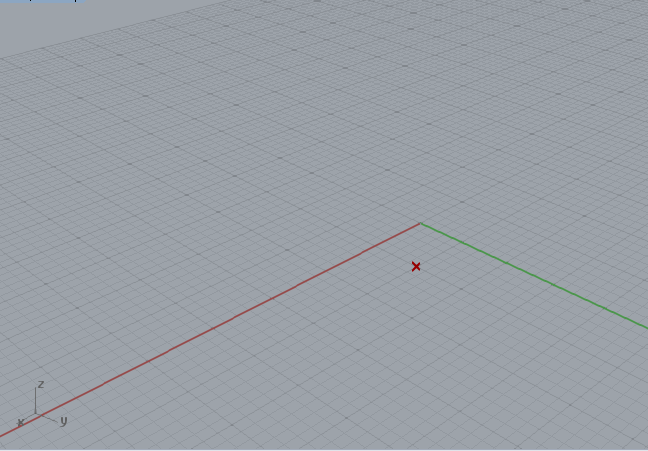
\includegraphics[width=.9\linewidth]{a01s00.png}
  \caption{Initial point}
  \label{fig:a01s00}
\end{subfigure}%
\begin{subfigure}{0.3\textwidth}
  \centering
  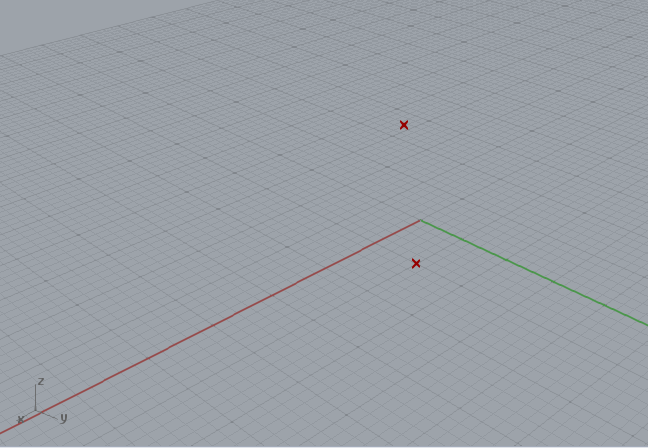
\includegraphics[width=.9\linewidth]{a01s01.png}
  \caption{Height point}
  \label{fig:a01s01}
\end{subfigure}
\begin{subfigure}{0.3\textwidth}
  \centering
  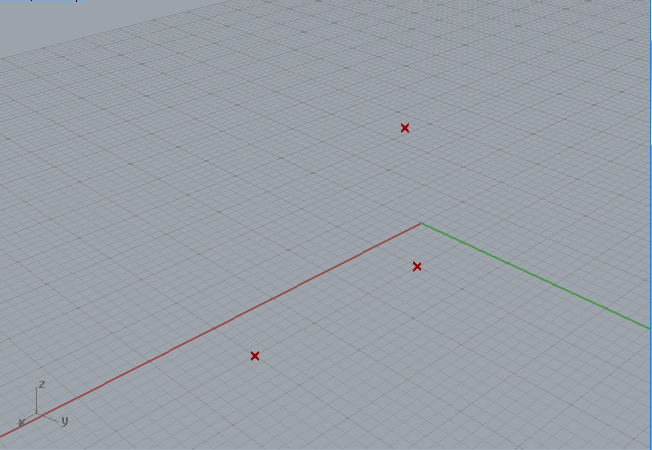
\includegraphics[width=.9\linewidth]{a01s02.png}
  \caption{Point on the base}
  \label{fig:a01s02}
\end{subfigure}


\begin{subfigure}{0.3\textwidth}
  \centering
  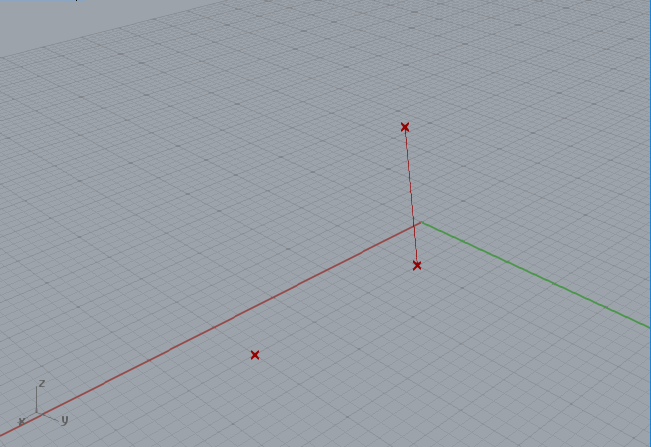
\includegraphics[width=.9\linewidth]{a01s03.png}
  \caption{Dome axis}
  \label{fig:a01s03}
\end{subfigure}
\begin{subfigure}{0.3\textwidth}
  \centering
  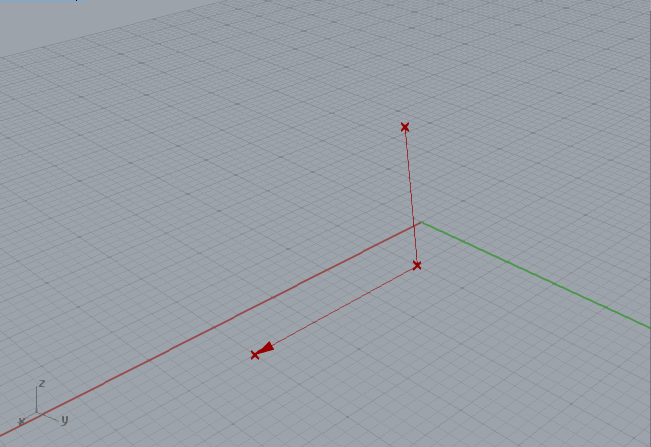
\includegraphics[width=.9\linewidth]{a01s04a.png}
  \caption{Auxiliary vector}
  \label{fig:a01s04a}
\end{subfigure}
\begin{subfigure}{0.3\textwidth}
  \centering
  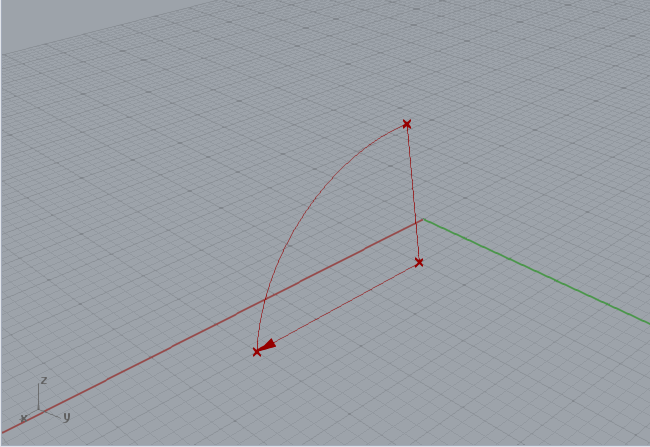
\includegraphics[width=.9\linewidth]{a01s04b.png}
  \caption{Petal arch}
  \label{fig:a01s04b}
\end{subfigure}


\begin{subfigure}{0.3\textwidth}
  \centering
  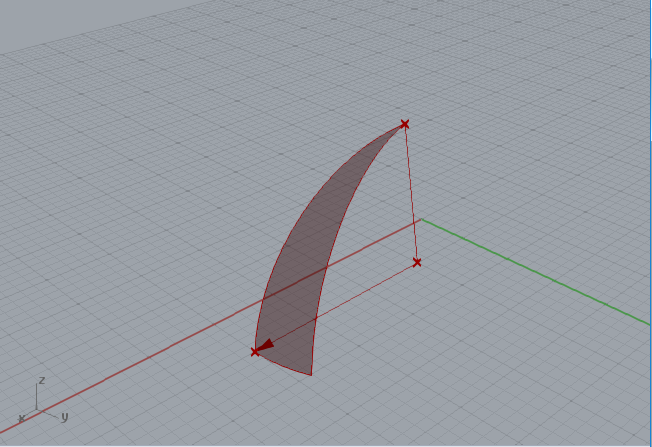
\includegraphics[width=.9\linewidth]{a01s06.png}
  \caption{Petal surface}
  \label{fig:a01s06}
\end{subfigure}
\begin{subfigure}{0.3\textwidth}
  \centering
  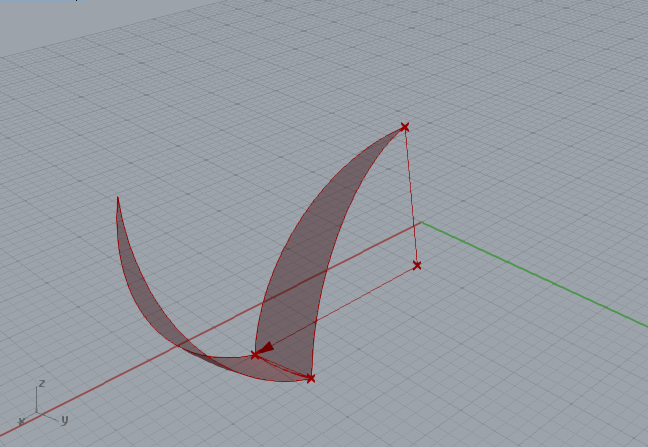
\includegraphics[width=.9\linewidth]{a01s08.png}
  \caption{Rotated petal}
  \label{fig:a01s08}
\end{subfigure}
\begin{subfigure}{0.3\textwidth}
  \centering
  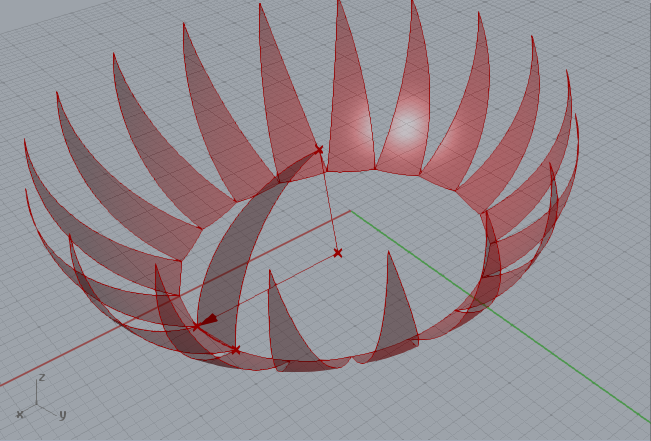
\includegraphics[width=.9\linewidth]{a01s09.png}
  \caption{Full dome}
  \label{fig:a01s09}
\end{subfigure}


\caption{Steps of the one petal algorithm}
\label{fig:a01steps}
\end{figure}

In a geometric constraint solver environment, the definition of the rules (constraints) can only be conceived by planning the geometric constructions. The first modeling strategy presented in this paper is: to model one petal, define a rotation axis (associated whit the rotation angle parameter) and copy it around a circle.Figure \ref{fig:a01steps} shows steps of the algorithm that will be discussed below.

Starting from the \textbf{center point} (fig. \ref{fig:a01s00}) of the base circle and making tow copies of the point: one in the $z$ axis, by the distance inputed in the cap height parameter, named as the \textbf{height point} (fig. \ref{fig:a01s01}); and the other in the $x$ axis, taking the value of the base radius as the module of the translation vector, referred as a \textbf{point on the base} (fig. \ref{fig:a01s02}). A line between the \textbf{base center} and the \textbf{height point} is also drawn, and will be called the \textbf{dome axis} (fig. \ref{fig:a01s03}).

The next step on drawing one petal is the arch on one side of it. As the arcs are drawn independently, the rules that define them should constraint the closed dome as a spherical cap. One of the ways to effectively constraint that construction is to make the arch tangent, in the height point, to a line or vector parallel to a direction defined as a line drawn from the base center to the point on base. In figure \ref{figura:tangente} that idea is illustrated, showing that only the blue arcs, that are tangent to the green vectors on the height point, form together a circle arch.


\begin{figure}[!h]
\begin{center}
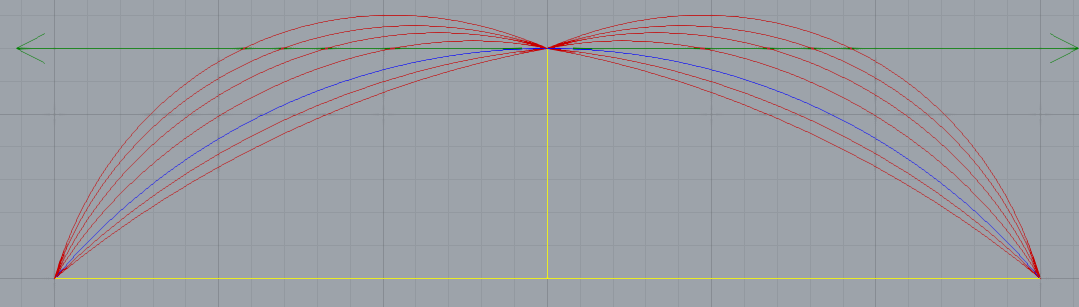
\includegraphics[width=0.65
\textwidth]{tangentes.png}
\caption{Constraining the arcs as part of a spherical cap}
\label{figura:tangente}
\end{center}
\end{figure}

In that step of the algorithm, an opportunity to debate some aspects of the geometric constructions applied in the process can be taken. More precisely, how this arcs can be defined by the classical geometric drawn and how this construction was translated to the computational environment. 

\begin{figure}[!h]
\begin{center}
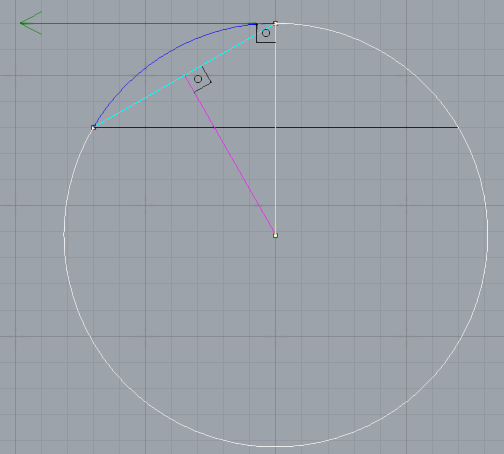
\includegraphics[width=0.5
\textwidth]{classicalarch.png}
\caption{Illustration of the traditional method for drawing the tangent arch}
\label{figura:classicalarch}
\end{center}
\end{figure}

The traditional steps to draw a tangent arch is illustrated in Figure \ref{figura:classicalarch}. The construction is based on two properties of circular arcs. One is that the tangent line in every point is perpendicular to the radius in that same point. The other is the most basic property of a circle, that every point on it is equidistant to the center.

Starting whit the two red points and the  tangent vector, represented by the green line in Figure \ref{figura:classicalarch}, and drawing a line perpendicular to the vector in the point that the vector tangency the arch, is safe to state that this perpendicular line (yellow) contains the center of the circle. The next step is to find a point on the perpendicular line that is equidistant to the two points of the arch. This can be done by drawing a segment that connects the tow points (cyan) and draw a perpendicular line in the middle of it (magenta). The point found by the intersection of the line perpendicular to the tangent vector and the line drawn in the middle point of the line that connect the two known points of the arch is equidistant (as are the sides of an isosceles triangle) to this points. So, with a compass centered in that intersection and starting form one of the known points to another, the arch can be defined (blue).

\begin{figure}[!h]
\begin{center}
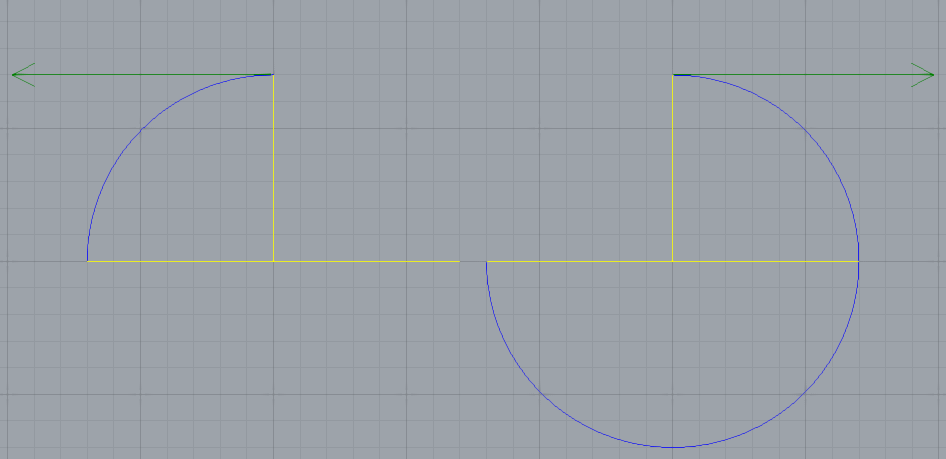
\includegraphics[width=0.5
\textwidth]{computationalarch.png}
\caption{Illustration of the computational method for drawing the tangent arch}
\label{figura:computationalarch}
\end{center}
\end{figure}

Is important to note that the withe arch in Figure \ref{figura:classicalarch} is also tangent to the vector and contains the two known points. The decision to draw one arch or the other, in that traditional method is purely human made, relaying on the understanding of the intended construction. Drawing an arch perpendicular to a line considers the line's orientation but not it´s sense. In the computational environment, when this method of drawing an arch based on two points and a line was implemented, the sense of the line is used to define the sense in witch the arch should be drawn. Figure \ref{figura:computationalarch} illustrated the arcs generated by the method with vectors that have the same direction and opposite senses.

In the proposed algorithm the reference vector is defined by an ordinated segment from the \textbf{base center} to the \textbf{point on the base} (fig. \ref{fig:a01s04a}). The command that generates an arch by tow points and a vector have, as inputs, the \textbf{height point}, the \textbf{point on the base}, and the vector of the tangent in the \textbf{height point}  (fig. \ref{fig:a01s04b}). Constructing the arch this way will constrain the closed dome to a spherical cap whit the height and base radius assuming the values defined by the respective parameters.

The petal is created as a ruled surface, generated by a rotation around the \textbf{dome axis} in an angle named as the \textbf{petal angle} (fig. \ref{fig:a01s06}). Dividing a $360 ^{\circ}$ angel ($2\times \pi $ in radians) by the \textbf{number of petals} the \textbf{petal angle} is numerically calculated. 

To simulate the pivoting movement that opens the dome, a rotation axis connecting the base points of the petal needs to be created. Task that could be performed  by rotating the \textbf{point on the base} around the \textbf{dome axis} taking the \textbf{petal angle} as the rotation amount. A line is drawn between the two points and is called the \textbf{pivot axis}.

The Petal surface is rotated around the \textbf{pivot axis} in an angle defined by the \textbf{pivot rotation} parameter (fig. \ref{fig:a01s08}). To complete the algorithm and generate the \textbf{full dome} (fig. \ref{fig:a01s09}), a polar array of the \textbf{rotated petal} is generated in a $360 ^{\circ}$ angle around the \textbf{dome axis} taking the number of petals as the number of the elements of the array.

\section{The code}
\label{code}

Although any programming language could virtually be used to implement the code, the CAD software Rhinoceros 3D (version 5.11) and it's plug-in Grasshopper (version 0.9.0076), a visual algorithm interface and a constraint solver, where chosen for the intuitive nature of programming thought the connection of graphical components, and the fact the forms will be created inside a CAD system able to conduct architectural projects.

\begin{figure}[!h]
\begin{center}
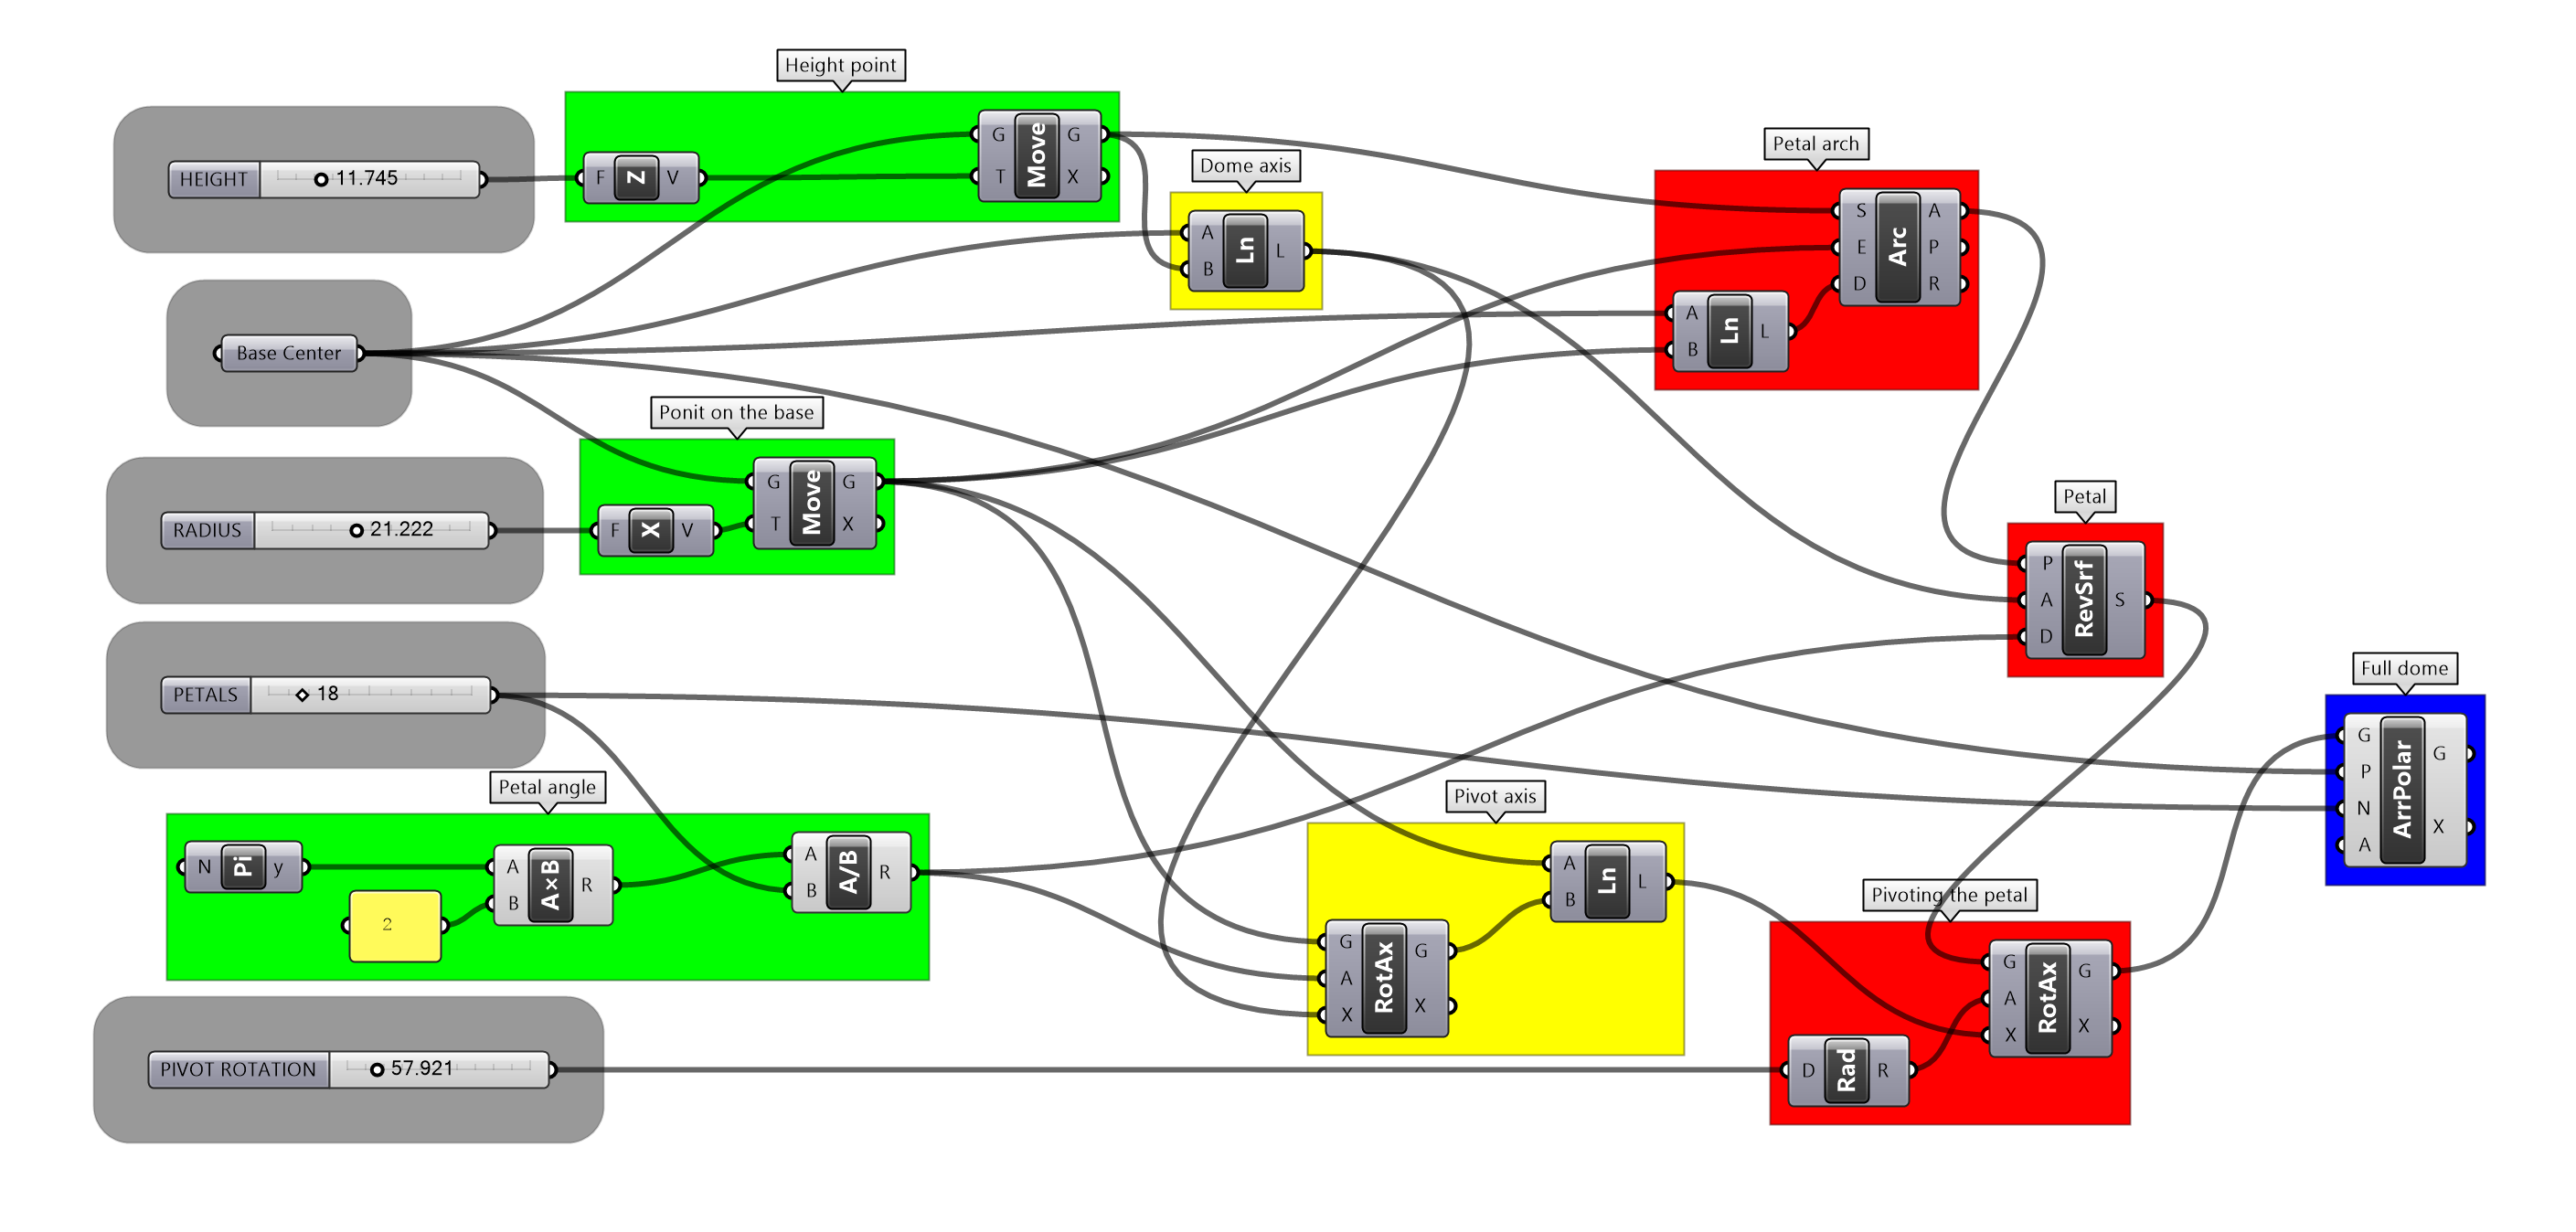
\includegraphics[width=0.95
\textwidth]{alg01.png}
\caption{One petal algorithm}
\label{figura:alg01}
\end{center}
\end{figure}

Figure \ref{figura:alg01} is the code implemented in the programming interface and also a flowchart of the algorithm. The data flows from left to right through the wire like connections between the components.

In the grey boxes are the parameters. From top to bottom: \textbf{height}, \textbf{base center},\textbf{ radius}, \textbf{number of petals} and \textbf{pivot rotation}. the top green box generates the \textbf{height point}, the middle green \textbf{the point on the base}, the bottom green calculates the \textbf{petal angle}. The yellow box on top generates the \textbf{dome axis} taking the \textbf{base center} and the \textbf{height point} as inputs, the bottom yellow outputs the \textbf{pivot axis}. The \textbf{auxiliary vector} and the \textbf{petal arch} are calculated in the top red box, the middle red box perform the revolution that generated de \textbf{petal surface} and the bottom red rotates it around the \textbf{pivot axis}. The blue box is responsible for the polar array operation that generates the \textbf{full dome}.



\section{List manipulation based algorithm}
\label{listmanip}

\begin{figure}
\begin{subfigure}{0.3\textwidth}
  \centering
  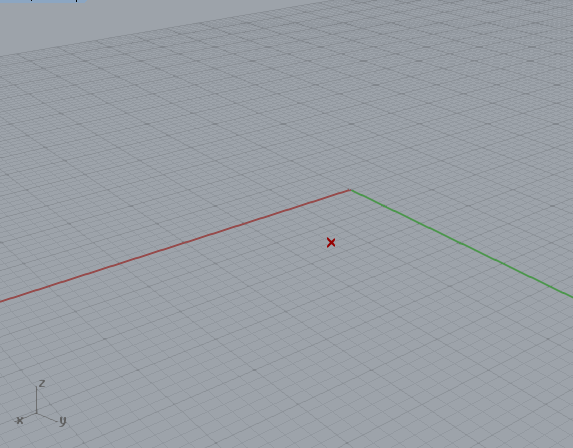
\includegraphics[width=.9\linewidth]{a02s00.png}
  \caption{Initial point}
  \label{fig:a02s01}
\end{subfigure}%
\begin{subfigure}{0.3\textwidth}
  \centering
  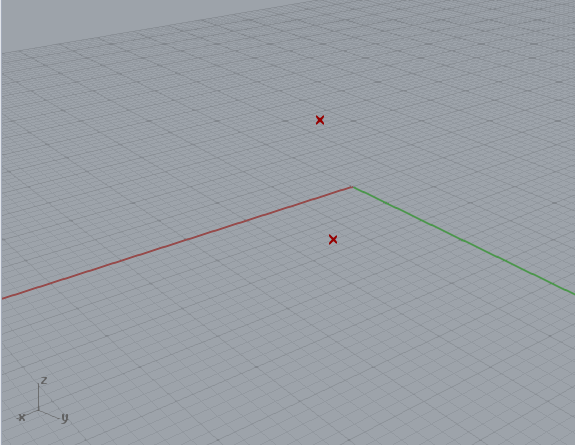
\includegraphics[width=.9\linewidth]{a02s01.png}
  \caption{Height point}
  \label{fig:a02s02}
\end{subfigure}
\begin{subfigure}{0.3\textwidth}
  \centering
  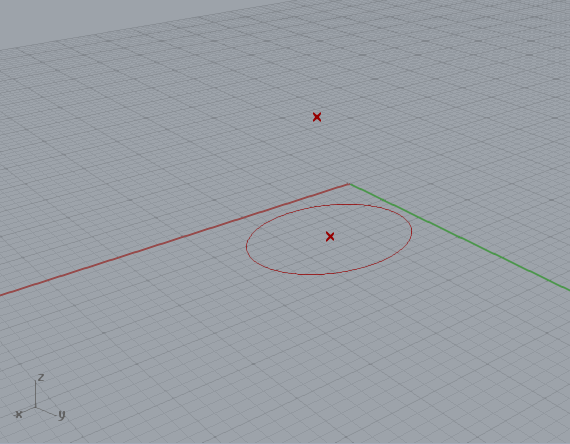
\includegraphics[width=.9\linewidth]{a02s03.png}
  \caption{Base circle}
  \label{fig:a02s03}
\end{subfigure}


\begin{subfigure}{0.3\textwidth}
  \centering
  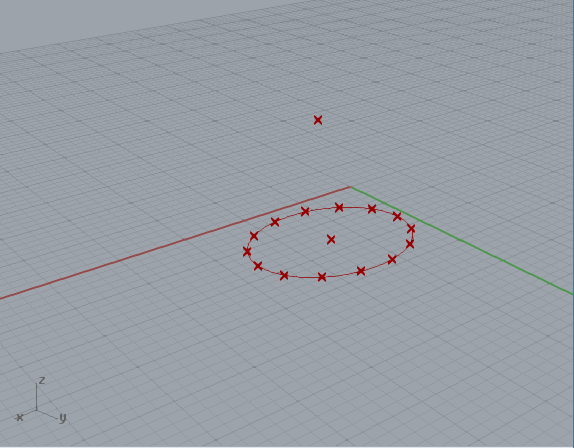
\includegraphics[width=.9\linewidth]{a02s04.png}
  \caption{Base points list}
  \label{fig:a02s04}
\end{subfigure}
\begin{subfigure}{0.3\textwidth}
  \centering
  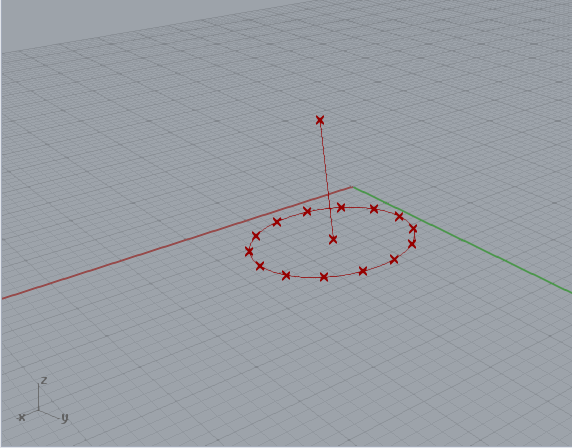
\includegraphics[width=.9\linewidth]{a02s05.png}
  \caption{Dome axis}
  \label{fig:a02s05}
\end{subfigure}
\begin{subfigure}{0.3\textwidth}
  \centering
  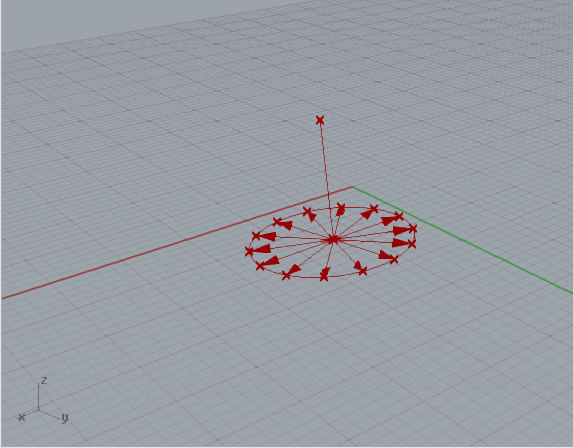
\includegraphics[width=.9\linewidth]{a02s06.png}
  \caption{Auxiliary vectors list}
  \label{fig:a02s06}
\end{subfigure}


\begin{subfigure}{0.3\textwidth}
  \centering
  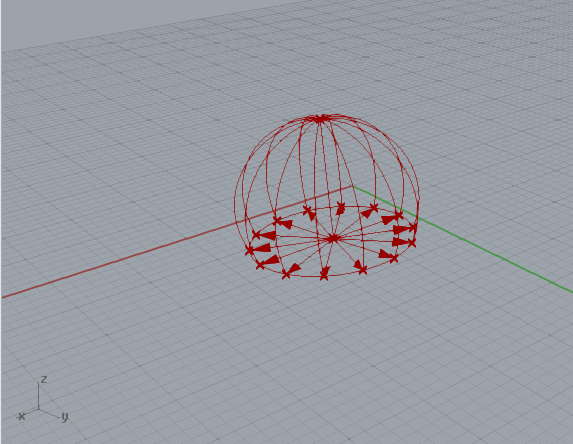
\includegraphics[width=.9\linewidth]{a02s07.png}
  \caption{Petals arcs list}
  \label{fig:a02s07}
\end{subfigure}
\begin{subfigure}{0.3\textwidth}
  \centering
  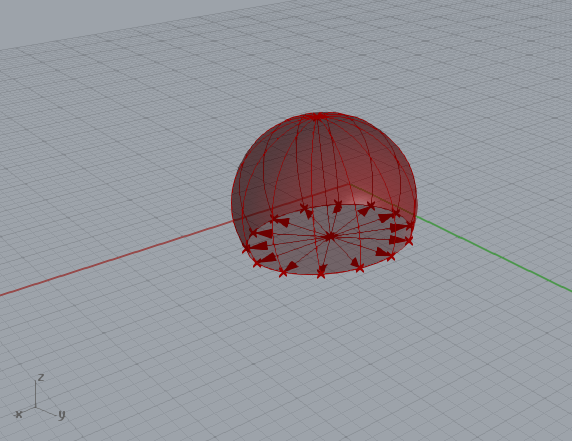
\includegraphics[width=.9\linewidth]{a02s08.png}
  \caption{Petals surfaces list}
  \label{fig:a02s08}
\end{subfigure}
\begin{subfigure}{0.3\textwidth}
  \centering
  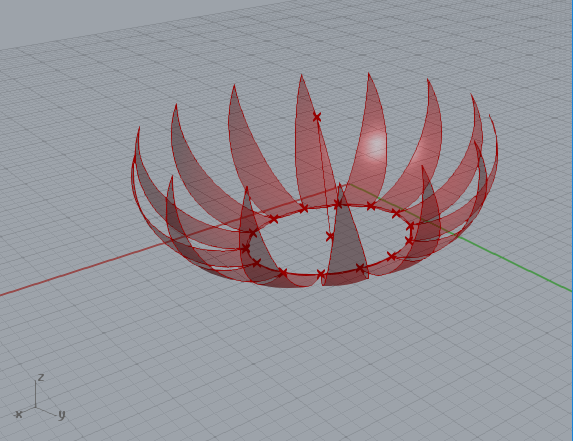
\includegraphics[width=.9\linewidth]{a02s09.png}
  \caption{Full dome}
  \label{fig:a02s09}
\end{subfigure}


\caption{Steps of the list manipulation based algorithm}
\label{fig:a02steps}
\end{figure}

The one petal algorithm presented in the previous sections satisfies the conditions and objectives of the proposed generative algorithm. Is an efficient and linear way of defining the rules. The list manipulation based programming strategies are current related do the Lisp programming paradigm proposed by John McCarthy in 1959 \cite{McCarthy1960}. Tightly associated whit the artificial intelligence field \cite{Steele:1996:EL:234286.1057818}, the list manipulation has also many applications in CAD environments. 

Taking as example a line creation command having as inputs points $A$ and $B$, drawing a line that goes from start point $A$ to end point $B$. If the second input is substituted by a list of points $B, C, D, E$, the result of this list operations e a list of lines $\bar{AB}, \bar{AC}, \bar{AD}$ and $\bar{AE}$, created by the application of a single line command. If two lists are used as inputs ($A, B, C, D, E$ and $F, G, H, I, J$) the result will be a list of lines between the equivalent points in each ordinated lists ($\bar{AF}, \bar{BG}, \bar{CH}, \bar{DI}$ and $\bar{EJ}$).

A variant implementation of the dome algorithm based on list programming is presented in this section to exemplify and introduce the concept. In the one petal algorithm example the steps generates one element at time, in the list manipulation based algorithm lists of elements will be created in a way that corresponding elements of every petal will be created simultaneously and all the petals will be generated and modified in parallel.

Figure \ref{fig:a02steps} shows the steps of the list manipulation based strategy, and starts from the \textbf{base center} (fig. \ref{fig:a02s01}) and creates the \textbf{height point} (fig. \ref{fig:a02s02}) in the same way it is created by the previous example. A circle is drawn using the \textbf{base center} and \textbf{base radius} parameters as inputs (fig. \ref{fig:a02s03}). The point on base of the first algorithm is replaced by a \textbf{base point list} (fig. \ref{fig:a02s04}), all of them constricted to the radius distance from the \textbf{base center}. The dome axis (fig. \ref{fig:a02s05}) is generated as it was in the previous rule set. In stead of a single vector, an auxiliary vectors lists (fig. \ref{fig:a02s06}) is generated by connecting the \textbf{base center} to the \textbf{base point list}. The \textbf{petal arcs list} (fig. \ref{fig:a02s07}) is drawn taking the \textbf{height point} as the start, the \textbf{base points list} as the end and the \textbf{auxiliary vectors list} as the tangents directions and sense.

\begin{figure}[!h]
\begin{center}
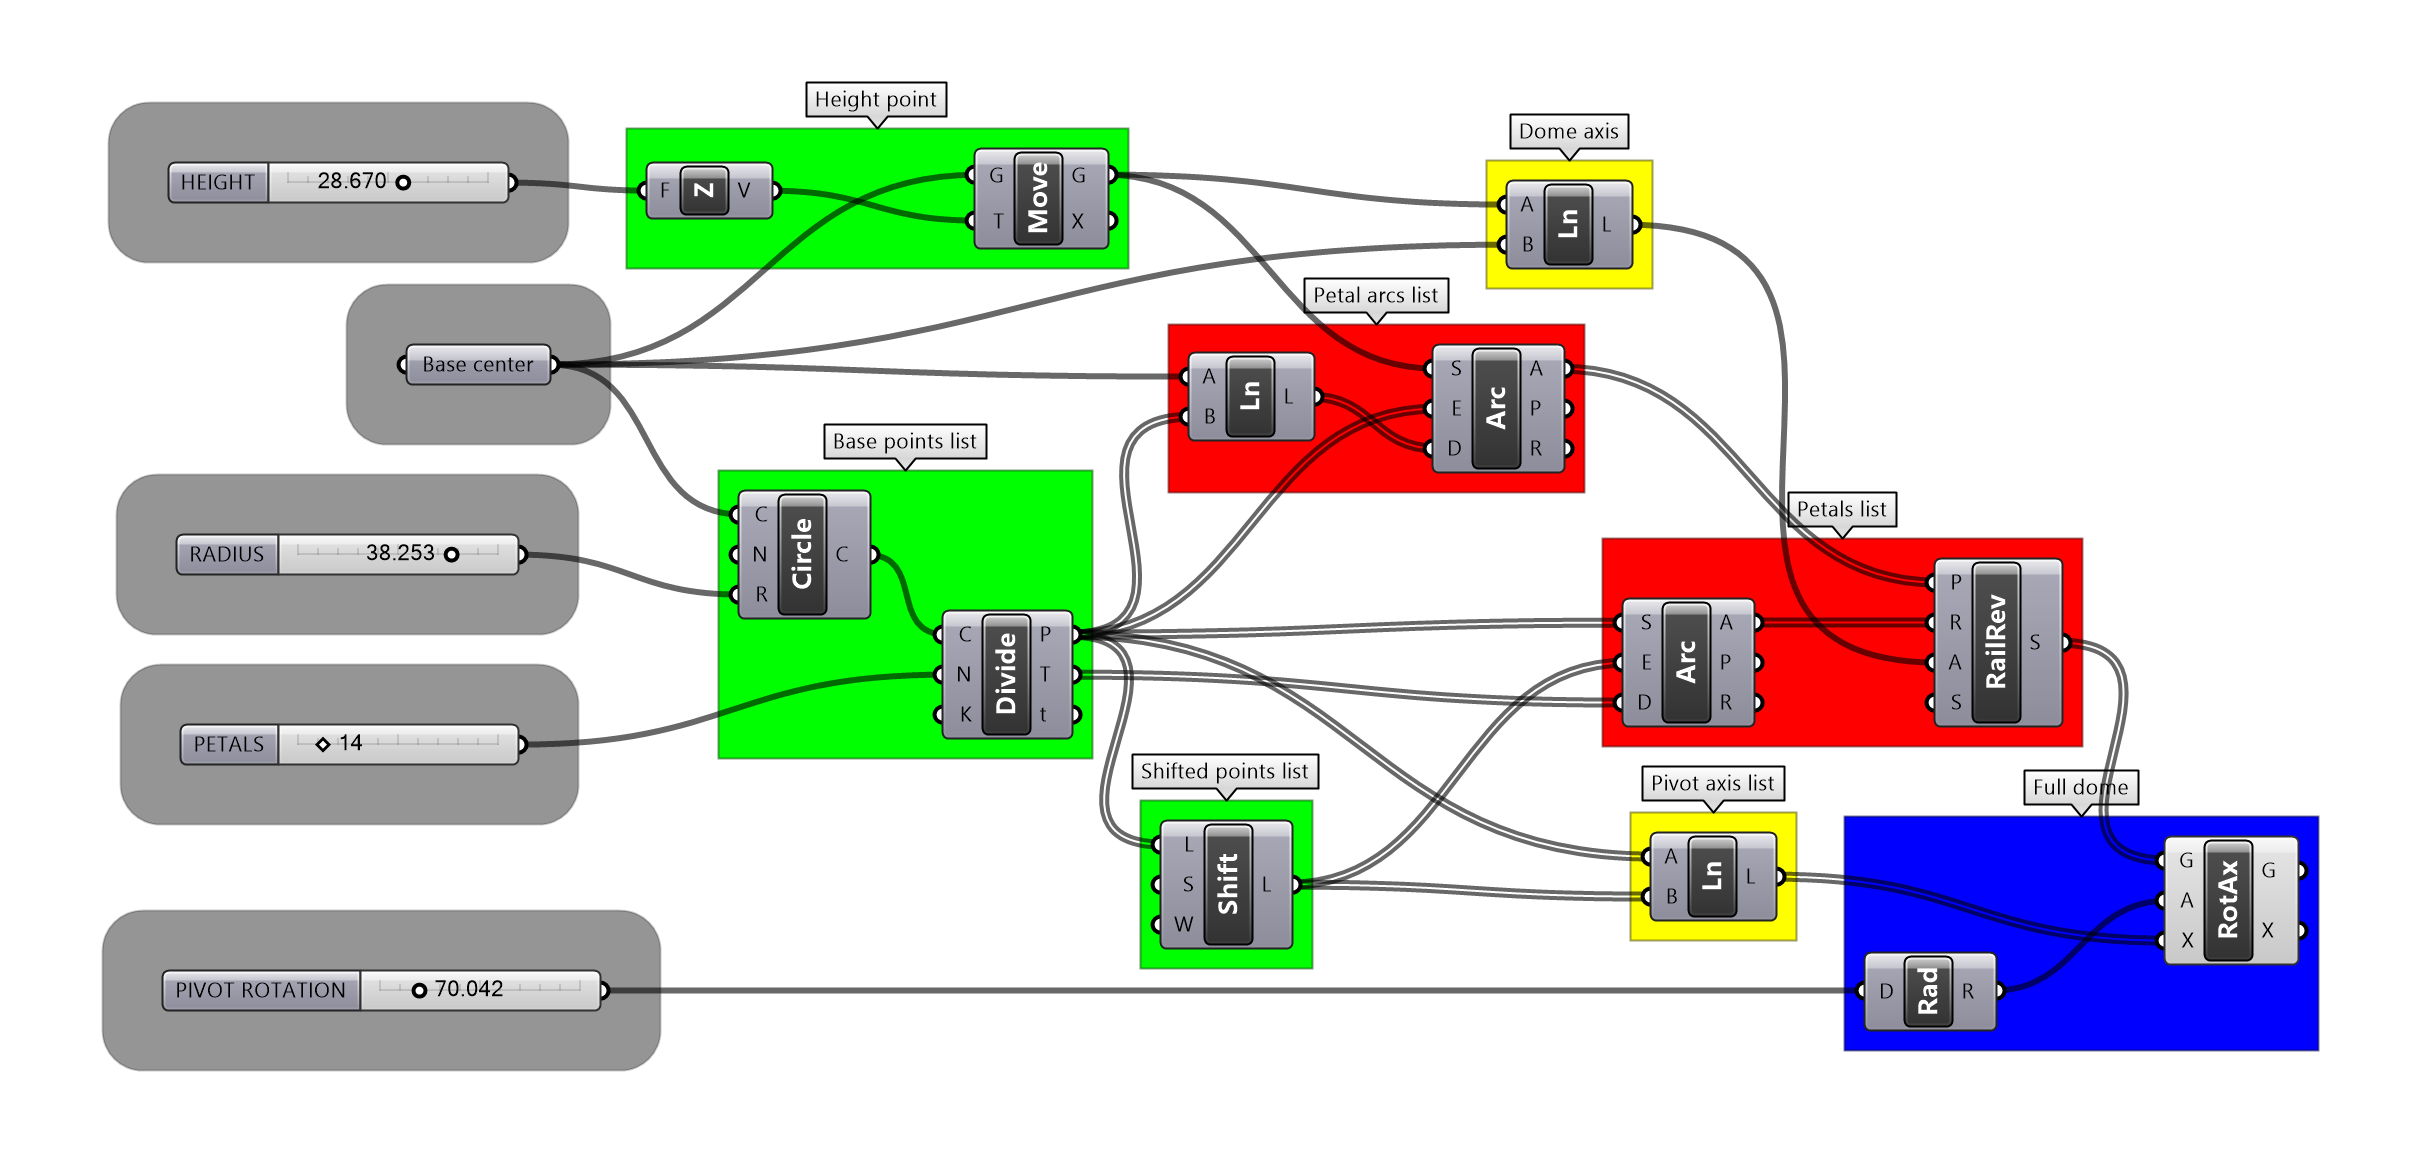
\includegraphics[width=0.95
\textwidth]{alg02.png}
\caption{List manipulation based algorithm}
\label{figura:alg02}
\end{center}
\end{figure}

Up to this point the ordinated lists are used to perform commands that operates on respective elements of the lists and no explicit manipulation was required. A simple but important operation on the \textbf{base points list} is part of the proposed rules, and is used to generate the forms and exemplify the applications of this programming methodology. The idea is to extract the first element of a list and append it back on the end. In a proposed points list represented as $A, B, C, D, E$, this operation will output $B, C, D, E, A$. Generating lines between the equivalent points in the two lists will result in a list of lines that connects adjacent points: ($\bar{AB}, \bar{BC}, \bar{CD}$ and $\bar{DE}$). In Figure \ref{figura:alg02} this operation is represented in the bottom green box, taking the \textbf{base points list} (middle green box) and outputting the \textbf{shifted points list}.

The \textbf{shifted points list} is directly used in two steps of the algorithm. The first is to create a \textbf{pivot axes list} by drawing lines between the \textbf{base points list} and the \textbf{shifted points list} (fig \ref{figura:alg02} bottom yellow box). The second is to generate auxiliary arcs to the \textbf{petal surface list} creation (fig \ref{figura:alg02} red bottom box). The middle green box on Figure \ref{figura:alg02} generates the \textbf{base points list} by dividing the \textbf{base circle} in the given \textbf{number of petals}, the grasshopper curve division component also outputs a list of the tangent vectors of the curve in the division points. Arcs are drawn whit start point provided by the \textbf{base points list}, end points defined by the correspondent elements in the \textbf{shifted points list}, and the sense and directions of the equivalent tangent vectors. This auxiliary arcs are used in replace of the \textbf{petal angle} in the first algorithm to define the revolution amount angle of the petals surface (fig \ref{figura:alg02} red bottom box) around the \textbf{dome axis} (fig \ref{figura:alg02} yellow top box).

The petals surface list (fig. \ref{fig:a02s08}) are rotated around the correspondent \textbf{pivot axes list} in the angle provided by the pivot rotation parameter, drawing the \textbf{full dome} (fig. \ref{fig:a02s09}).

\section{Analysing the algorithms outputs}
\label{outs01}

\begin{figure}[h]
\begin{subfigure}{0.3\textwidth}
  \centering
  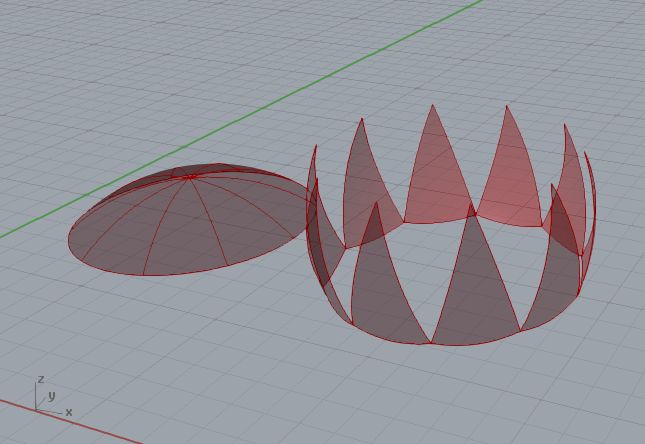
\includegraphics[width=.9\linewidth]{dome01.png}
  \caption{}
  \label{fig:dome01}
\end{subfigure}%
\begin{subfigure}{0.3\textwidth}
  \centering
  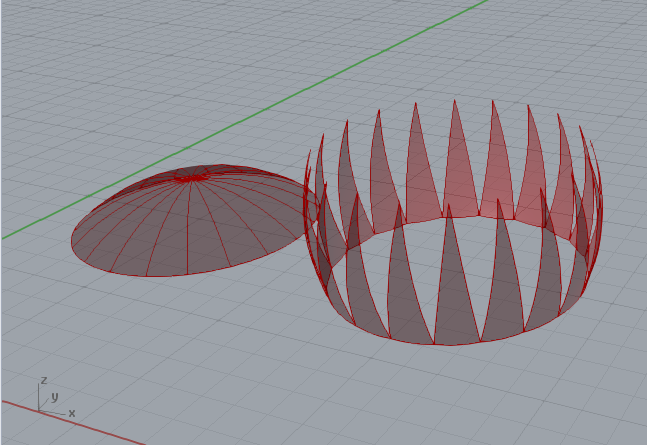
\includegraphics[width=.9\linewidth]{dome02.png}
  \caption{}
  \label{fig:dome02}
\end{subfigure}
\begin{subfigure}{0.3\textwidth}
  \centering
  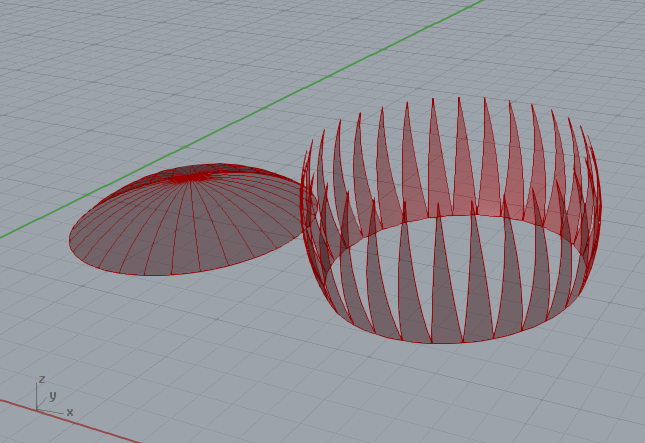
\includegraphics[width=.9\linewidth]{dome03.png}
  \caption{}
  \label{fig:dome03}
\end{subfigure}


\begin{subfigure}{0.3\textwidth}
  \centering
  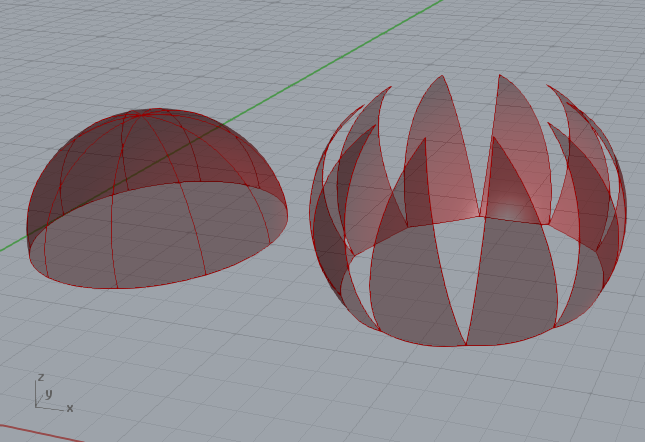
\includegraphics[width=.9\linewidth]{dome04.png}
  \caption{}
  \label{fig:dome04}
\end{subfigure}
\begin{subfigure}{0.3\textwidth}
  \centering
  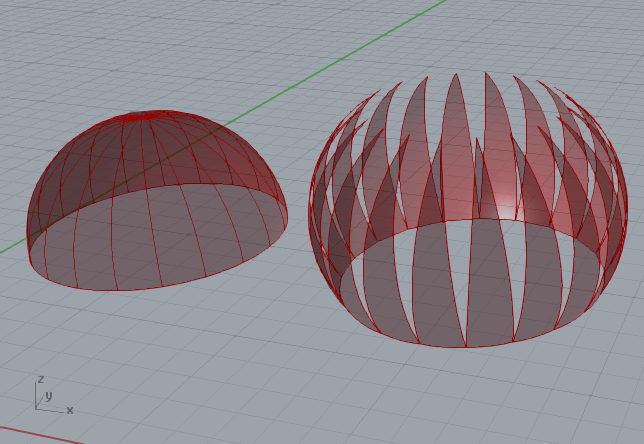
\includegraphics[width=.9\linewidth]{dome05.png}
  \caption{}
  \label{fig:dome05}
\end{subfigure}
\begin{subfigure}{0.3\textwidth}
  \centering
  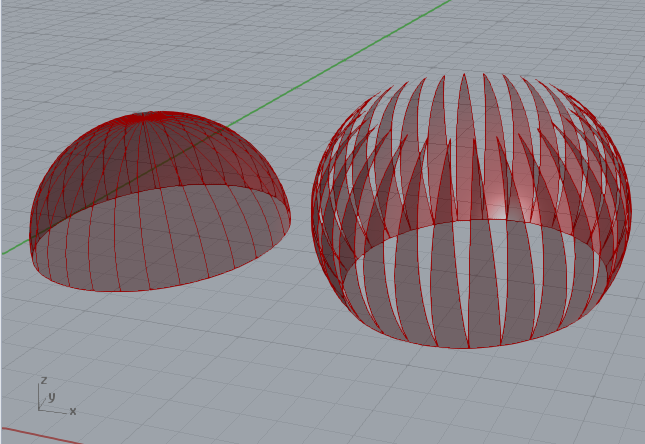
\includegraphics[width=.9\linewidth]{dome06.png}
  \caption{}
  \label{fig:dome06}
\end{subfigure}


\begin{subfigure}{0.3\textwidth}
  \centering
  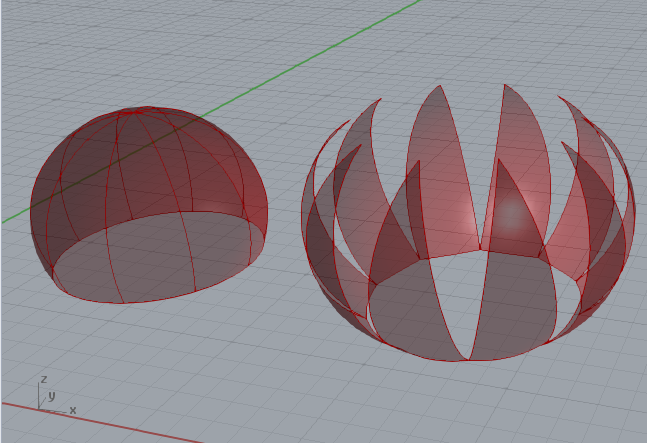
\includegraphics[width=.9\linewidth]{dome07.png}
  \caption{}
  \label{fig:dome07}
\end{subfigure}
\begin{subfigure}{0.3\textwidth}
  \centering
  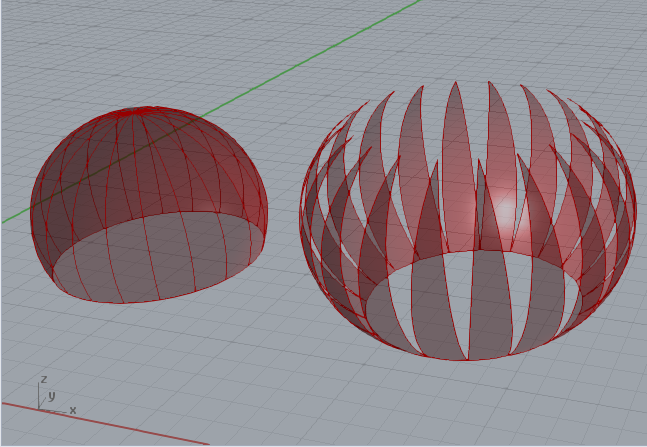
\includegraphics[width=.9\linewidth]{dome08.png}
  \caption{}
  \label{fig:dome08}
\end{subfigure}
\begin{subfigure}{0.3\textwidth}
  \centering
  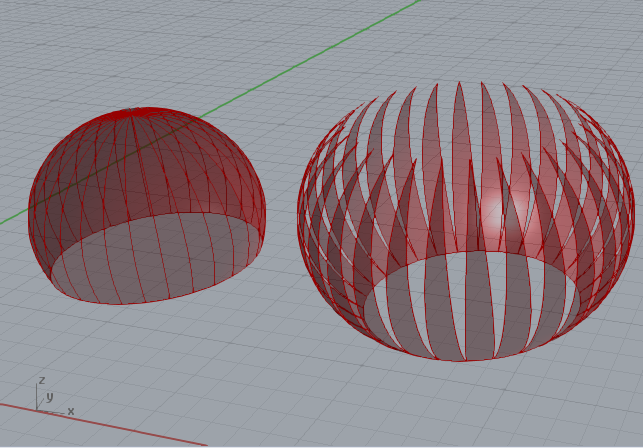
\includegraphics[width=.9\linewidth]{dome09.png}
  \caption{}
  \label{fig:dome09}
\end{subfigure}


\caption{Variant domes created by the algorithms}
\label{fig:domeresult}
\end{figure}

The flowchart in Figure \ref{figura:fluxogramametodologia}, after the idea is established, the rules are planned, the code is implemented and a first is generated by the first set of parameters; the designer is in charge of evaluate the result, reset the parameters and/or modify the code and continuously repeat this operations until a constructive form ends up being elected as the one to be build.

Figure \ref{fig:domeresult} shows a set of solutions generated exclusively by modifications made over the values of the parameters. One of the decisions that the designer should made is the size of the \textbf{base radius}, strongly related to amount of light and dynamics of the air that should circulate in and out of the building it is attached on. This evaluation could relay on the designer's experience and intuition or calculations that could be performed whit ou without the aid of computational analyses tools. Since the variations of the forms are automatically generated, a tool that analyses 3D models tends to be more efficient for the task.

Not only the building itself, but the characteristics of the environment should be considered in this choosing process, but some relations between the parameters result in relevant changes in the outputted geometries. In the first row of Figure \ref{fig:domeresult} the domes have bigger values for the \textbf{base radius} than the ones of the \textbf{height} parameter, the second line shows equal values and in the third row the \textbf{radius} is smaller than the \textbf{height}. This fact could be easily demonstrated geometrically, but can also be experimented by the parameters modifications. 

The aesthetic perception of the different simulations can be observed in the images of figure \ref{fig:domeresult} but is better understood when compared to the domes and respective buildings of Figures \ref{figura:sarah} and \ref{figura:trt}. The first one presents a bigger value for the \textbf{height} parameter than the \textbf{radius}, producing a fluid relation between the curves of the building's forms and the dome as a finishing element. An inverted configuration of parameters in the relations between this values will generate a brusque or even flat interruption on the forms composition. In the second, the domes adopts a more discreet elevation from it's base, dialogging with the almost flat roof solution of the buildings.

Wile the quantitative investigations can be numerically evaluated, the qualitative aspects, as the aesthetics, can only be approached and addressed by the raising and answering of some loosely defined questions. The simple analysis proposed aims to exemplify how this subjectives requisitions can be handled by the generative algorithm's methodology.


\section{Modifying the code}
\label{extrap}

\begin{figure}[h]
\begin{subfigure}{0.3\textwidth}
  \centering
  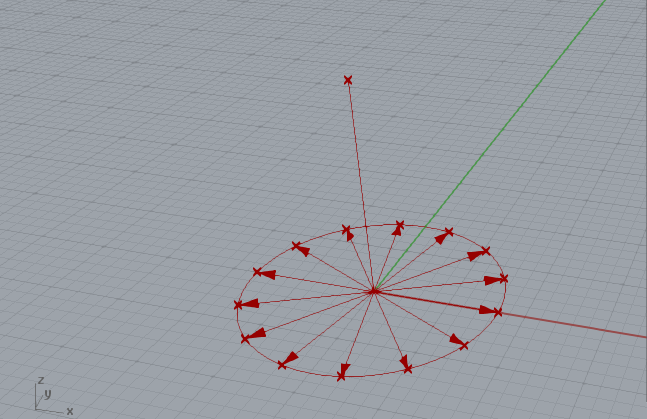
\includegraphics[width=.9\linewidth]{ag03s01.png}
  \caption{Auxiliary vectors list}
  \label{fig:ag03s01}
\end{subfigure}%
\begin{subfigure}{0.3\textwidth}
  \centering
  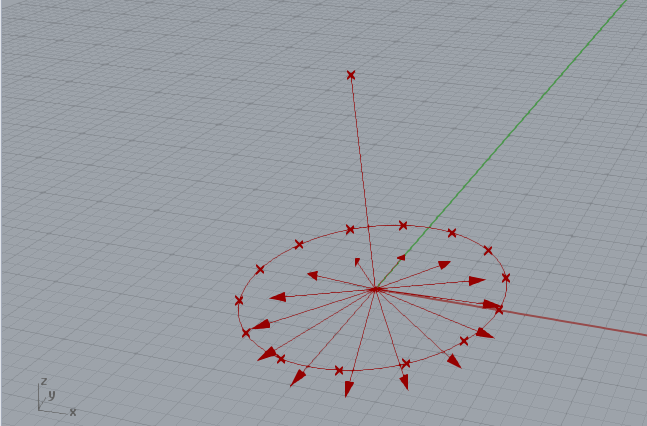
\includegraphics[width=.9\linewidth]{ag03s02.png}
  \caption{Rotated tangents list}
  \label{fig:ag03s02}
\end{subfigure}
\begin{subfigure}{0.3\textwidth}
  \centering
  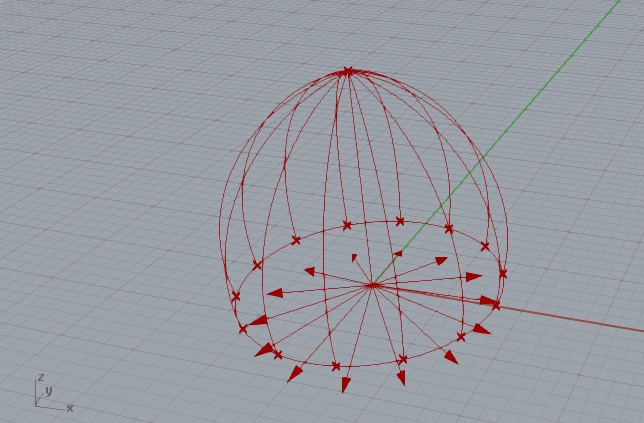
\includegraphics[width=.9\linewidth]{ag03s03.png}
  \caption{Petals arcs lists}
  \label{fig:ag03s03}
\end{subfigure}

\caption{Steps of the lancet dome algorithm}
\label{fig:lancetdome}
\end{figure}

Modifications in the parameters are the fastest way of generating alternative results in a generative design system. The results registered in Figure \ref{fig:domeresult} could be generated by both of the algorithms presented, but the flowchart in Figure \ref{figura:fluxogramametodologia} foresees that the code and the rules could be also modified in the scope of this work methodology. To illustrate this possibility some changes in the list manipulation based algorithm are proposed to enable the code to create not only spherical cap domes, but also geometries derived from lancet arcs.




Few modifications are need to complete this task. The steps presented in Figure \ref{fig:a02steps} are followed in the exact order until the \textbf{auxiliary vectors} are created (fig \ref{fig:a02s06}). Then the vectors suffer a rotation defined by a new parameter called \textbf{tangent rotation} and the \textbf{petals arcs list} is created taking this new vectors as inputs. After that,\textbf{ the petals surface} list and the \textbf{full dome} are created by the same procedures represented in figures \ref{fig:a02s08} and \ref{fig:a02s09}.



\begin{figure}[h]
\begin{subfigure}{0.3\textwidth}
  \centering
  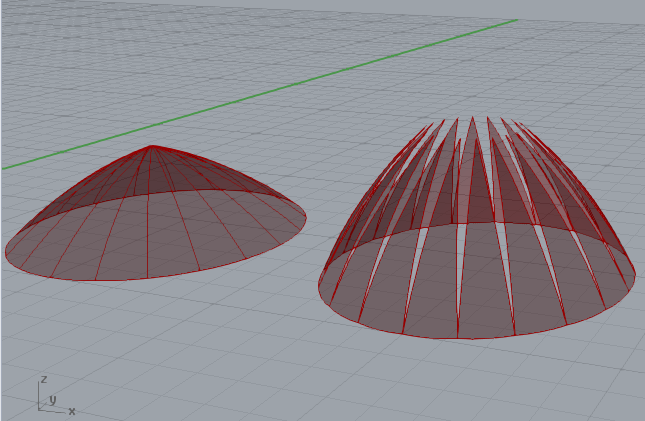
\includegraphics[width=.9\linewidth]{lancetDome01.png}
  \caption{}
  \label{fig:lancetDome01}
\end{subfigure}%
\begin{subfigure}{0.3\textwidth}
  \centering
  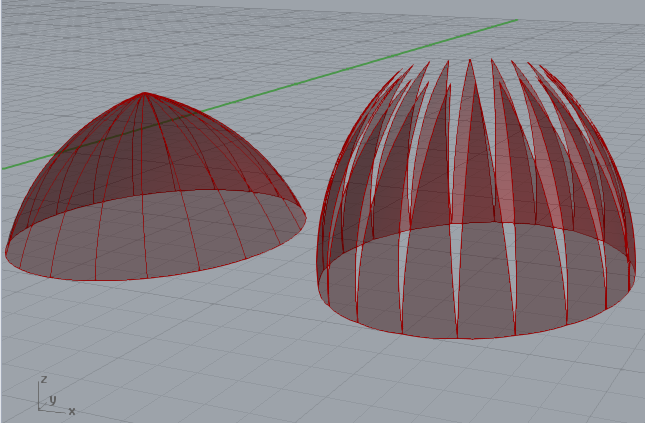
\includegraphics[width=.9\linewidth]{lancetDome02.png}
  \caption{}
  \label{fig:lancetDome02}
\end{subfigure}
\begin{subfigure}{0.3\textwidth}
  \centering
  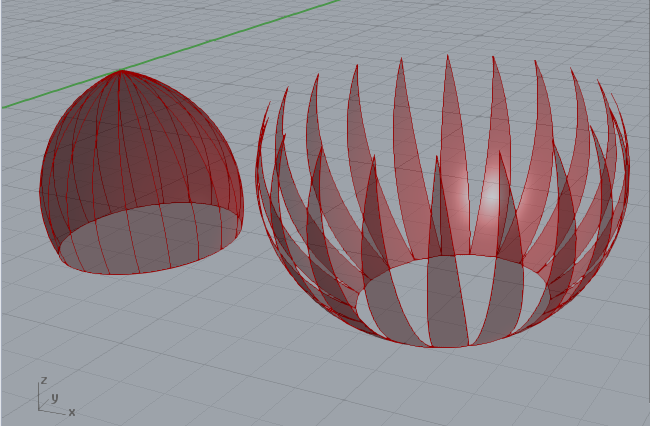
\includegraphics[width=.9\linewidth]{lancetDome03.png}
  \caption{}
  \label{fig:lancetDome03}
\end{subfigure}

\caption{Steps of the lancet dome algorithm}
\label{fig:lancetdomeexamples}
\end{figure}

If the tangent rotation parameter is equal to zero, the results are constrained to geometries similar to the ones presented in Figure \ref{fig:domeresult}, else they assume the pointed end of a lancet arch as Figure \ref{fig:lancetdomeexamples} illustrates.

\begin{figure}[!h]
\begin{center}
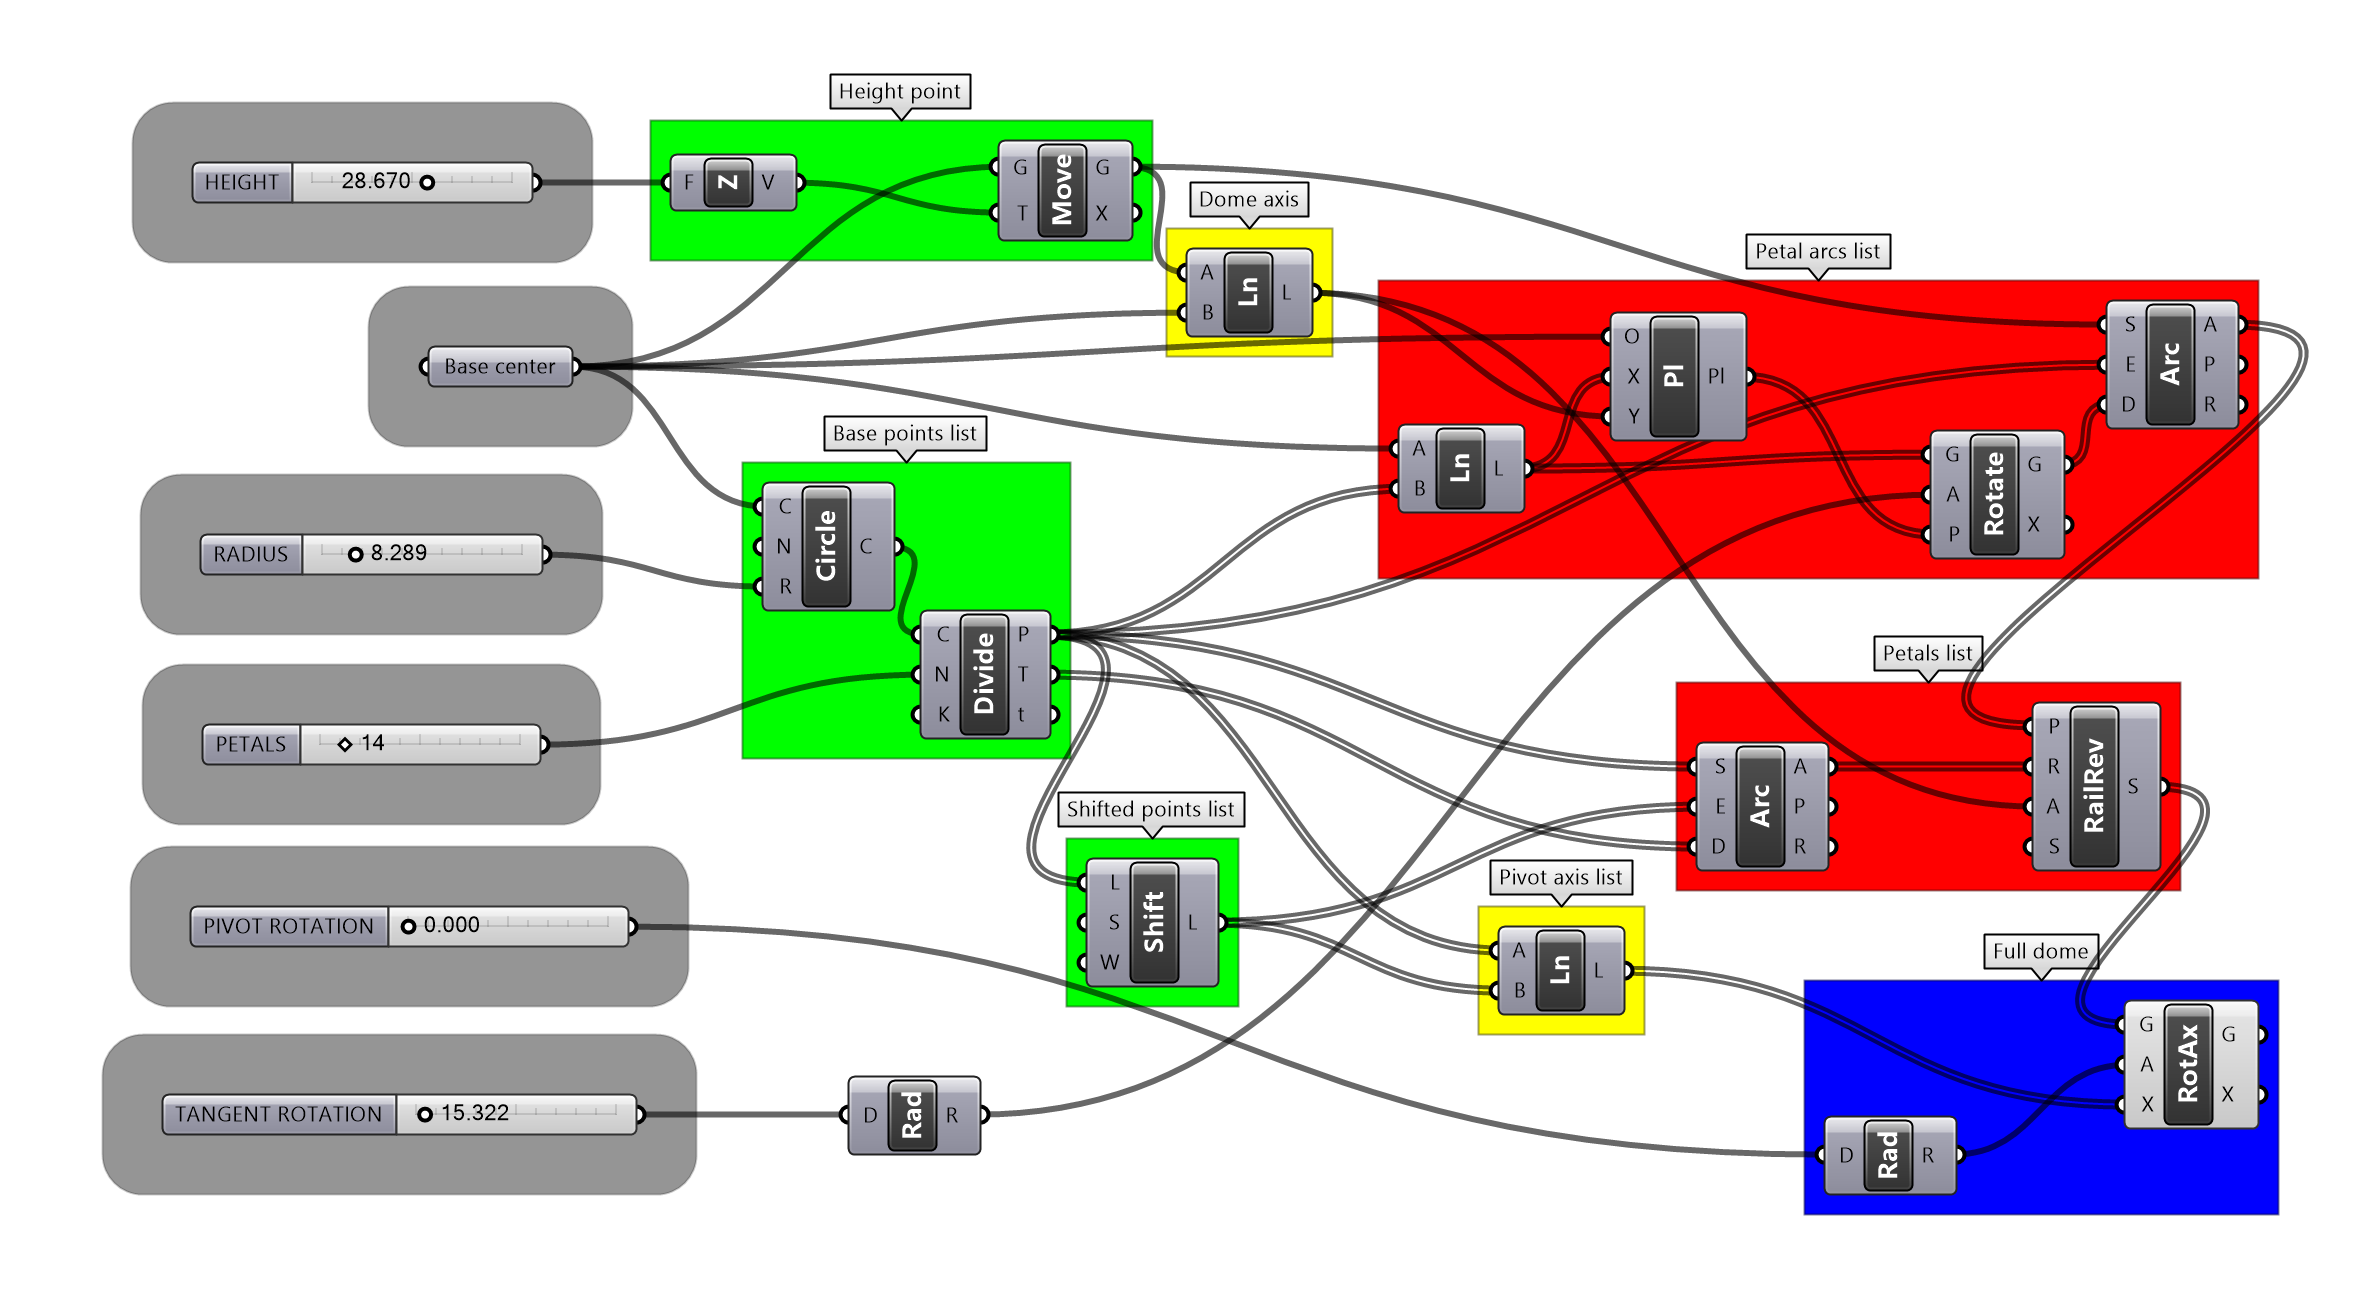
\includegraphics[width=0.95
\textwidth]{alg03.png}
\caption{Lancet arch algorithm}
\label{figura:alg03}
\end{center}
\end{figure}

The visual code presented in Figure \ref{figura:alg03} presents this changes in comparison with Figure \ref{figura:alg02}. The \textbf{tangent rotation} parameter is added (bottom grey box) and the \textbf{auxiliary vectors} are rotated around the $z$ axes of a list of planes created with origin in the \textbf{base center} $x$ axes along the direction and sense of the \textbf{auxiliary vectors} and $y$ axes following the \textbf{dome axis} oriented line, this rotated tangents list is inputed as the vector required by the \textbf{petals arcs list} creation component (top red box). 


\section{Conclusion}
\label{conc}

The proposed exercise discussed along this article succeed in approaching the basics aspects of the generative design methodology, encompassing all the possible variants of the flowchart in Figure \ref{figura:fluxogramametodologia}, explaining the most important geometric constructions used, providing an overview of some programming procedures and presenting how the election of constructive forms could be performed in both qualitative and quantitative aspects.

The one sentence definition of the idea purposely omits the fact that, in that stage of the analysis of the domes references, they are all spherical caps. If that was stated, the modification of the algorithm in section \ref{extrap} will also modify the idea. Although this modification is not described by the flowchart (fig. \ref{figura:fluxogramametodologia}) it is indeed a possible movement in the work process of a generative algorithm. Since code reuse is a common programming activity, the case of a stated characteristic of an idea been modified along the way should not me treated as an issue, but as a natural possibility.

The interdisciplinary nature of Architecture meets an also interdisciplinary domain that a comprehensive understanding of the generative design systems demand. The scope of all the different disciplines interrelated in this exercise was not by far covered, but the effort of bringing those notions together in a coherent context should guide future works of presenting the subject and a virtuous way of establishing new discussions on the secular field of Architecture.


%\appendix

%\section{Implemented test algorithms}
%\label{appendix-sec1}



%% References
%%
%% Following citation commands can be used in the body text:
%% Usage of \cite is as follows:
%%   \cite{key}         ==>>  [#]
%%   \cite[chap. 2]{key} ==>> [#, chap. 2]
%%

%% References with bibTeX database:

\bibliographystyle{elsarticle-num}
% \bibliographystyle{elsarticle-harv}
% \bibliographystyle{elsarticle-num-names}
% \bibliographystyle{model1a-num-names}
% \bibliographystyle{model1b-num-names}
% \bibliographystyle{model1c-num-names}
% \bibliographystyle{model1-num-names}
% \bibliographystyle{model2-names}
% \bibliographystyle{model3a-num-names}
% \bibliographystyle{model3-num-names}
% \bibliographystyle{model4-names}
% \bibliographystyle{model5-names}
% \bibliographystyle{model6-num-names}

\bibliography{library}


\end{document}

%%
%% End of file `elsarticle-template-num.tex'.
